\documentclass[twoside]{book}

% Packages required by doxygen
\usepackage{fixltx2e}
\usepackage{calc}
\usepackage{doxygen}
\usepackage[export]{adjustbox} % also loads graphicx
\usepackage{graphicx}
\usepackage[utf8]{inputenc}
\usepackage{makeidx}
\usepackage{multicol}
\usepackage{multirow}
\PassOptionsToPackage{warn}{textcomp}
\usepackage{textcomp}
\usepackage[nointegrals]{wasysym}
\usepackage[table]{xcolor}

% Font selection
\usepackage[T1]{fontenc}
\usepackage[scaled=.90]{helvet}
\usepackage{courier}
\usepackage{amssymb}
\usepackage{sectsty}
\renewcommand{\familydefault}{\sfdefault}
\allsectionsfont{%
  \fontseries{bc}\selectfont%
  \color{darkgray}%
}
\renewcommand{\DoxyLabelFont}{%
  \fontseries{bc}\selectfont%
  \color{darkgray}%
}
\newcommand{\+}{\discretionary{\mbox{\scriptsize$\hookleftarrow$}}{}{}}

% Page & text layout
\usepackage{geometry}
\geometry{%
  a4paper,%
  top=2.5cm,%
  bottom=2.5cm,%
  left=2.5cm,%
  right=2.5cm%
}
\tolerance=750
\hfuzz=15pt
\hbadness=750
\setlength{\emergencystretch}{15pt}
\setlength{\parindent}{0cm}
\setlength{\parskip}{3ex plus 2ex minus 2ex}
\makeatletter
\renewcommand{\paragraph}{%
  \@startsection{paragraph}{4}{0ex}{-1.0ex}{1.0ex}{%
    \normalfont\normalsize\bfseries\SS@parafont%
  }%
}
\renewcommand{\subparagraph}{%
  \@startsection{subparagraph}{5}{0ex}{-1.0ex}{1.0ex}{%
    \normalfont\normalsize\bfseries\SS@subparafont%
  }%
}
\makeatother

% Headers & footers
\usepackage{fancyhdr}
\pagestyle{fancyplain}
\fancyhead[LE]{\fancyplain{}{\bfseries\thepage}}
\fancyhead[CE]{\fancyplain{}{}}
\fancyhead[RE]{\fancyplain{}{\bfseries\leftmark}}
\fancyhead[LO]{\fancyplain{}{\bfseries\rightmark}}
\fancyhead[CO]{\fancyplain{}{}}
\fancyhead[RO]{\fancyplain{}{\bfseries\thepage}}
\fancyfoot[LE]{\fancyplain{}{}}
\fancyfoot[CE]{\fancyplain{}{}}
\fancyfoot[RE]{\fancyplain{}{\bfseries\scriptsize Generated by Doxygen }}
\fancyfoot[LO]{\fancyplain{}{\bfseries\scriptsize Generated by Doxygen }}
\fancyfoot[CO]{\fancyplain{}{}}
\fancyfoot[RO]{\fancyplain{}{}}
\renewcommand{\footrulewidth}{0.4pt}
\renewcommand{\chaptermark}[1]{%
  \markboth{#1}{}%
}
\renewcommand{\sectionmark}[1]{%
  \markright{\thesection\ #1}%
}

% Indices & bibliography
\usepackage{natbib}
\usepackage[titles]{tocloft}
\setcounter{tocdepth}{3}
\setcounter{secnumdepth}{5}
\makeindex

% Hyperlinks (required, but should be loaded last)
\usepackage{ifpdf}
\ifpdf
  \usepackage[pdftex,pagebackref=true]{hyperref}
\else
  \usepackage[ps2pdf,pagebackref=true]{hyperref}
\fi
\hypersetup{%
  colorlinks=true,%
  linkcolor=blue,%
  citecolor=blue,%
  unicode%
}

% Custom commands
\newcommand{\clearemptydoublepage}{%
  \newpage{\pagestyle{empty}\cleardoublepage}%
}

\usepackage{caption}
\captionsetup{labelsep=space,justification=centering,font={bf},singlelinecheck=off,skip=4pt,position=top}

%===== C O N T E N T S =====

\begin{document}

% Titlepage & ToC
\hypersetup{pageanchor=false,
             bookmarksnumbered=true,
             pdfencoding=unicode
            }
\pagenumbering{alph}
\begin{titlepage}
\vspace*{7cm}
\begin{center}%
{\Large Mopatop\+Tests }\\
\vspace*{1cm}
{\large Generated by Doxygen 1.8.14}\\
\end{center}
\end{titlepage}
\clearemptydoublepage
\pagenumbering{roman}
\tableofcontents
\clearemptydoublepage
\pagenumbering{arabic}
\hypersetup{pageanchor=true}

%--- Begin generated contents ---
\chapter{Main Page}
\label{index}\hypertarget{index}{}\hypertarget{index_intro_sec}{}\section{Introduction}\label{index_intro_sec}
This directory contains the unit tests for the mopatop model \hypertarget{index_Main}{}\subsection{Main ideas}\label{index_Main}
The system uses the cppunit test system, version 1.\+14 to test each part of the model against some standard cases~\newline
For each class in the model, a header file is defined here containing tests of that class. Each header containes~\newline
a test suite, each of which runs through some of the methods defined in the classes to check that behave as expected~\newline
in a well defined and limited number of cases where the output can be known ahead of time. This helps to prevent some~\newline
of the more easily caught programming or conceptual errors. Each test suite is added to a test\+Runner defined in \mbox{\hyperlink{testing_8cpp}{testing.\+cpp}} ~\newline
Note that because some of the classes can depend on each other, running some of the tests might potentially affect others~\newline
(e.\+g. the time\+Step class is static, so if its parameters are altered, subsequent tests that depend on the timestep might~\newline
be altered). This should be borne in mind when writing new tests.~\newline
When modifications are made to any of the classes, tests should be re-\/run to chekc that nothing has been broken. Any new~\newline
code not subject to testing should have tests added here as necessary. The tests themsevles have their own documentation~\newline
generated by Doxygen and kept in the html sub-\/directory. \hypertarget{index_Compiling}{}\subsection{Compiling}\label{index_Compiling}
On a linux system with g++ installed just do ~\newline
g++ -\/otests -\/fopenmp -\/std=c++17 -\/lcppunit ../timestep.cpp ../places.cpp ../disease.cpp ../schedulelist.cpp ../agent.cpp \mbox{\hyperlink{testing_8cpp}{testing.\+cpp}}~\newline
Note the current version requires g++$>$= and c++17 in order for the filesystem function to work (for creating new directories etc.)~\newline
\hypertarget{index_Run}{}\subsection{Running}\label{index_Run}
At present this is a simple command-\/line application -\/ just type the executable name (tests above) and then return.~\newline
This will use the parameter file called test\+Parameter\+File in this directory. ~\newline

\begin{DoxyCode}
./tests
\end{DoxyCode}
 The parameter file allows for a number of tests that depend on parameter settings. \hypertarget{index_Details}{}\subsection{Details}\label{index_Details}
A test\+Runner is defined from the Cpp\+Unit\+::\+Text\+Ui\+::\+Test\+Runner class. Each of the testsuites is added to this using 
\begin{DoxyCode}
runner.addTest( testClass::suite() );
\end{DoxyCode}
 where test\+Class is defined in one of the header files. Each header file uses the C\+P\+P\+U\+N\+I\+T\+\_\+\+T\+E\+S\+T\+\_\+\+S\+U\+I\+TE macro to define a testsuite~\newline
which is a set of functions, each function containing one or more tests 
\begin{DoxyCode}
 CPPUNIT\_TEST\_SUITE( testClass );
\textcolor{comment}{//add tests defined below}
CPPUNIT\_TEST( function1 );
CPPUNIT\_TEST( function2 );
CPPUNIT\_TEST\_SUITE\_END();
\end{DoxyCode}
 If needed a set\+Up() and tear\+Down() function can be added, which will automatically create and destroy variables afresh at the start of~\newline
each test function, provided the class inherits from Cpp\+Unit\+::\+Test\+Fixture e.\+g. 
\begin{DoxyCode}
\textcolor{keyword}{class }\mbox{\hyperlink{classplaceTest}{placeTest}} : \textcolor{keyword}{public} CppUnit::TestFixture  \{
  place* \mbox{\hyperlink{classplaceTest_a0f4e660bdadc034488490bbadc33e09f}{p}};
\textcolor{keyword}{public}:
 \textcolor{comment}{//persistent objects to use during testing}
 \textcolor{keywordtype}{void} \mbox{\hyperlink{classplaceTest_a1818bbe31325c6d9344b35f3b510cacf}{setUp}}()
 \{
     \mbox{\hyperlink{classplaceTest_a0f4e660bdadc034488490bbadc33e09f}{p}} = \textcolor{keyword}{new} place();
 \}
 
 \textcolor{keywordtype}{void} \mbox{\hyperlink{classplaceTest_a2a0d52566e44cc385dc8fecdae504d6f}{tearDown}}() 
 \{
     \textcolor{keyword}{delete} \mbox{\hyperlink{classplaceTest_a0f4e660bdadc034488490bbadc33e09f}{p}};
 \}
 \};
\end{DoxyCode}
 NB these function defintions must come B\+E\+F\+O\+RE the above testsuite defintions.~\newline
In the test function typically asserts are used to check the result of of a test e.\+g. 
\begin{DoxyCode}
\textcolor{keywordtype}{void} function1()
\{
    \textcolor{comment}{//default ID is zero}
    CPPUNIT\_ASSERT(0==p->getID());
    \}
\end{DoxyCode}
 These are pass/fail tests, and will be reported giving the text of the failed test and line number in the code if needed~\newline
In addition tests may report text to stdout where required. Note the uses here of the pre-\/defined pointer p from the set\+Up().~\newline
Variables can also be defined as needed within each test function however.~\newline
An output directory is generated afresh (and any previous values are overwritten) each time the tests are run contains ~\newline
 a small amount of data for checiking output works as expected.. 
\chapter{mopatop tests}
\label{md_README}
\Hypertarget{md_README}
This directory contains the unit test suites for the mopatop model. See html/index.\+html for documentation 
\chapter{Hierarchical Index}
\section{Class Hierarchy}
This inheritance list is sorted roughly, but not completely, alphabetically\+:\begin{DoxyCompactList}
\item Test\+Fixture\begin{DoxyCompactList}
\item \contentsline{section}{agent\+Test}{\pageref{classagentTest}}{}
\item \contentsline{section}{disease\+Test}{\pageref{classdiseaseTest}}{}
\item \contentsline{section}{model\+Factory\+Test}{\pageref{classmodelFactoryTest}}{}
\item \contentsline{section}{model\+Test}{\pageref{classmodelTest}}{}
\item \contentsline{section}{parameter\+Test}{\pageref{classparameterTest}}{}
\item \contentsline{section}{place\+Test}{\pageref{classplaceTest}}{}
\item \contentsline{section}{random\+Test}{\pageref{classrandomTest}}{}
\item \contentsline{section}{schedule\+List\+Test}{\pageref{classscheduleListTest}}{}
\item \contentsline{section}{time\+Reporter\+Test}{\pageref{classtimeReporterTest}}{}
\item \contentsline{section}{time\+Step\+Test}{\pageref{classtimeStepTest}}{}
\item \contentsline{section}{travel\+Schedule\+Test}{\pageref{classtravelScheduleTest}}{}
\end{DoxyCompactList}
\item Text\+Test\+Progress\+Listener\begin{DoxyCompactList}
\item \contentsline{section}{My\+Custom\+Progress\+Test\+Listener}{\pageref{classMyCustomProgressTestListener}}{}
\end{DoxyCompactList}
\end{DoxyCompactList}

\chapter{Class Index}
\section{Class List}
Here are the classes, structs, unions and interfaces with brief descriptions\+:\begin{DoxyCompactList}
\item\contentsline{section}{\mbox{\hyperlink{classagentTest}{agent\+Test}} \\*Test out the agent class }{\pageref{classagentTest}}{}
\item\contentsline{section}{\mbox{\hyperlink{classdiseaseTest}{disease\+Test}} \\*Test the disease static classs }{\pageref{classdiseaseTest}}{}
\item\contentsline{section}{\mbox{\hyperlink{classmodelFactoryTest}{model\+Factory\+Test}} \\*Test out the model\+Factory class }{\pageref{classmodelFactoryTest}}{}
\item\contentsline{section}{\mbox{\hyperlink{classmodelTest}{model\+Test}} \\*Test out the model class }{\pageref{classmodelTest}}{}
\item\contentsline{section}{\mbox{\hyperlink{classMyCustomProgressTestListener}{My\+Custom\+Progress\+Test\+Listener}} \\*Report the start of each test }{\pageref{classMyCustomProgressTestListener}}{}
\item\contentsline{section}{\mbox{\hyperlink{classparameterTest}{parameter\+Test}} \\*Check parameter defaults are as expected }{\pageref{classparameterTest}}{}
\item\contentsline{section}{\mbox{\hyperlink{classplaceTest}{place\+Test}} \\*Check places for contamination levels and agent occupancy }{\pageref{classplaceTest}}{}
\item\contentsline{section}{\mbox{\hyperlink{classrandomTest}{random\+Test}} \\*Test some of the random number generator behaviour }{\pageref{classrandomTest}}{}
\item\contentsline{section}{\mbox{\hyperlink{classscheduleListTest}{schedule\+List\+Test}} \\*Test out the newclass class }{\pageref{classscheduleListTest}}{}
\item\contentsline{section}{\mbox{\hyperlink{classtimeReporterTest}{time\+Reporter\+Test}} \\*Check intervals are computed and reported as expected }{\pageref{classtimeReporterTest}}{}
\item\contentsline{section}{\mbox{\hyperlink{classtimeStepTest}{time\+Step\+Test}} \\*Check the class that maps the time step to a given set of real-\/world units (e.\+g. hours) }{\pageref{classtimeStepTest}}{}
\item\contentsline{section}{\mbox{\hyperlink{classtravelScheduleTest}{travel\+Schedule\+Test}} \\*Exercise the fixed travel schedules }{\pageref{classtravelScheduleTest}}{}
\end{DoxyCompactList}

\chapter{File Index}
\section{File List}
Here is a list of all documented files with brief descriptions\+:\begin{DoxyCompactList}
\item\contentsline{section}{\mbox{\hyperlink{agenttest_8h}{agenttest.\+h}} \\*File containing the definition of the \mbox{\hyperlink{classagentTest}{agent\+Test}} class }{\pageref{agenttest_8h}}{}
\item\contentsline{section}{\mbox{\hyperlink{diseasetest_8h}{diseasetest.\+h}} \\*File containing the definition of the \mbox{\hyperlink{classdiseaseTest}{disease\+Test}} class }{\pageref{diseasetest_8h}}{}
\item\contentsline{section}{\mbox{\hyperlink{modelfactorytest_8h}{modelfactorytest.\+h}} \\*File containing the definition of the \mbox{\hyperlink{classmodelFactoryTest}{model\+Factory\+Test}} class }{\pageref{modelfactorytest_8h}}{}
\item\contentsline{section}{\mbox{\hyperlink{modeltest_8h}{modeltest.\+h}} \\*File containing the definition of the \mbox{\hyperlink{classmodelTest}{model\+Test}} class }{\pageref{modeltest_8h}}{}
\item\contentsline{section}{\mbox{\hyperlink{parametertest_8h}{parametertest.\+h}} \\*File containing the definition of the \mbox{\hyperlink{classparameterTest}{parameter\+Test}} class for testing the parameter file }{\pageref{parametertest_8h}}{}
\item\contentsline{section}{\mbox{\hyperlink{placetest_8h}{placetest.\+h}} \\*File containing the definition of the \mbox{\hyperlink{classplaceTest}{place\+Test}} class }{\pageref{placetest_8h}}{}
\item\contentsline{section}{\mbox{\hyperlink{randomtest_8h}{randomtest.\+h}} \\*File containing the definition of the \mbox{\hyperlink{classrandomTest}{random\+Test}} class for the random number wrapper }{\pageref{randomtest_8h}}{}
\item\contentsline{section}{\mbox{\hyperlink{schedulelisttest_8h}{schedulelisttest.\+h}} \\*File containing the definition of the newclass\+Test class }{\pageref{schedulelisttest_8h}}{}
\item\contentsline{section}{\mbox{\hyperlink{testing_8cpp}{testing.\+cpp}} \\*Define the progress test listener, \mbox{\hyperlink{classMyCustomProgressTestListener}{My\+Custom\+Progress\+Test\+Listener}}, and the main function to run all the tests }{\pageref{testing_8cpp}}{}
\item\contentsline{section}{\mbox{\hyperlink{timereportertest_8h}{timereportertest.\+h}} \\*File containing the definition of the \mbox{\hyperlink{classtimeReporterTest}{time\+Reporter\+Test}} class for reporting run-\/time intervals }{\pageref{timereportertest_8h}}{}
\item\contentsline{section}{\mbox{\hyperlink{timesteptest_8h}{timesteptest.\+h}} \\*File containing the definition of the \mbox{\hyperlink{classtimeStepTest}{time\+Step\+Test}} class for checking the time step to real world times class is working }{\pageref{timesteptest_8h}}{}
\item\contentsline{section}{\mbox{\hyperlink{travelscheduletest_8h}{travelscheduletest.\+h}} \\*Test out the travel schedules using \mbox{\hyperlink{classtravelScheduleTest}{travel\+Schedule\+Test}} class }{\pageref{travelscheduletest_8h}}{}
\end{DoxyCompactList}

\chapter{Class Documentation}
\hypertarget{classagentTest}{}\section{agent\+Test Class Reference}
\label{classagentTest}\index{agent\+Test@{agent\+Test}}


test out the agent class  




{\ttfamily \#include $<$agenttest.\+h$>$}



Inheritance diagram for agent\+Test\+:\nopagebreak
\begin{figure}[H]
\begin{center}
\leavevmode
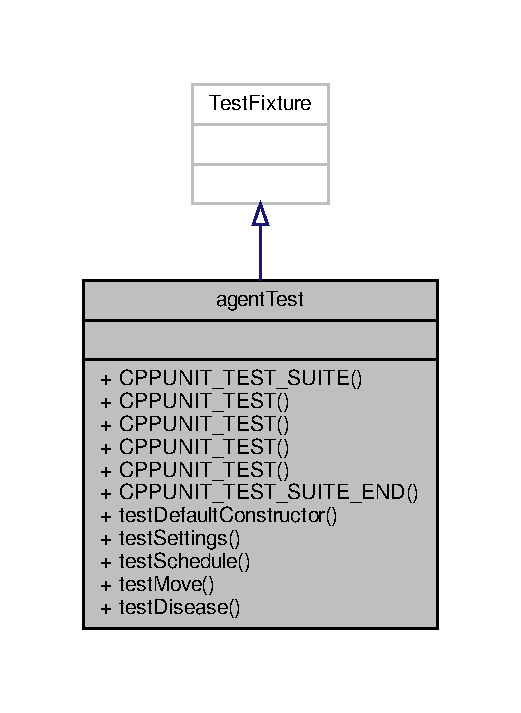
\includegraphics[width=250pt]{classagentTest__inherit__graph}
\end{center}
\end{figure}


Collaboration diagram for agent\+Test\+:\nopagebreak
\begin{figure}[H]
\begin{center}
\leavevmode
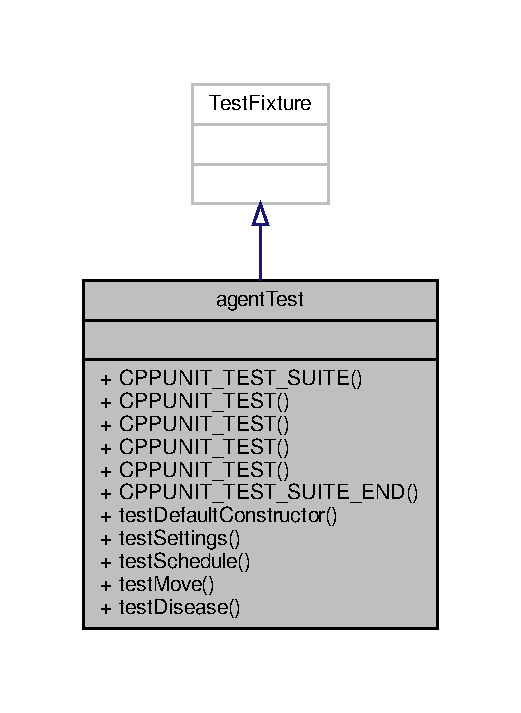
\includegraphics[width=250pt]{classagentTest__coll__graph}
\end{center}
\end{figure}
\subsection*{Public Member Functions}
\begin{DoxyCompactItemize}
\item 
\mbox{\Hypertarget{classagentTest_a948c6b1acfe35387e5c64612baa946b5}\label{classagentTest_a948c6b1acfe35387e5c64612baa946b5}} 
\mbox{\hyperlink{classagentTest_a948c6b1acfe35387e5c64612baa946b5}{C\+P\+P\+U\+N\+I\+T\+\_\+\+T\+E\+S\+T\+\_\+\+S\+U\+I\+TE}} (\mbox{\hyperlink{classagentTest}{agent\+Test}})
\begin{DoxyCompactList}\small\item\em automatically create a test suite to add tests to \end{DoxyCompactList}\item 
\mbox{\Hypertarget{classagentTest_af781fb1217505d9383a1d0f7de6da73f}\label{classagentTest_af781fb1217505d9383a1d0f7de6da73f}} 
\mbox{\hyperlink{classagentTest_af781fb1217505d9383a1d0f7de6da73f}{C\+P\+P\+U\+N\+I\+T\+\_\+\+T\+E\+ST}} (\mbox{\hyperlink{classagentTest_ade6fc2895d439529b21d4fb725302b77}{test\+Default\+Constructor}})
\begin{DoxyCompactList}\small\item\em test the default constructor \end{DoxyCompactList}\item 
\mbox{\Hypertarget{classagentTest_a85678ef4ae878bc43397deae1bdd2b44}\label{classagentTest_a85678ef4ae878bc43397deae1bdd2b44}} 
\mbox{\hyperlink{classagentTest_a85678ef4ae878bc43397deae1bdd2b44}{C\+P\+P\+U\+N\+I\+T\+\_\+\+T\+E\+ST}} (\mbox{\hyperlink{classagentTest_ad39e9d21138b56f55a29ced6fdba8e58}{test\+Settings}})
\begin{DoxyCompactList}\small\item\em test some of the set/get functions \end{DoxyCompactList}\item 
\mbox{\Hypertarget{classagentTest_a4b0cf2b0288ecd554a74ee8e5c1f2338}\label{classagentTest_a4b0cf2b0288ecd554a74ee8e5c1f2338}} 
\mbox{\hyperlink{classagentTest_a4b0cf2b0288ecd554a74ee8e5c1f2338}{C\+P\+P\+U\+N\+I\+T\+\_\+\+T\+E\+ST}} (\mbox{\hyperlink{classagentTest_a628c4b06eee5b0e6e7a45c842ed70429}{test\+Disease}})
\begin{DoxyCompactList}\small\item\em test the disease functions \end{DoxyCompactList}\item 
\mbox{\Hypertarget{classagentTest_a6558275101998971b56abdd2a323623d}\label{classagentTest_a6558275101998971b56abdd2a323623d}} 
\mbox{\hyperlink{classagentTest_a6558275101998971b56abdd2a323623d}{C\+P\+P\+U\+N\+I\+T\+\_\+\+T\+E\+ST}} (\mbox{\hyperlink{classagentTest_adaa25e2c092be46311aea330d19d7f94}{test\+Schedule}})
\begin{DoxyCompactList}\small\item\em test the schedule \end{DoxyCompactList}\item 
\mbox{\hyperlink{classagentTest_a51ff7b623cb89bce6fa8bab5f8af04b7}{C\+P\+P\+U\+N\+I\+T\+\_\+\+T\+E\+S\+T\+\_\+\+S\+U\+I\+T\+E\+\_\+\+E\+ND}} ()
\begin{DoxyCompactList}\small\item\em test occupancy lists \end{DoxyCompactList}\item 
void \mbox{\hyperlink{classagentTest_ade6fc2895d439529b21d4fb725302b77}{test\+Default\+Constructor}} ()
\begin{DoxyCompactList}\small\item\em make sure default agent has no disease, is alive, and knows about 3 kinds of place. Check ID increments. \end{DoxyCompactList}\item 
\mbox{\Hypertarget{classagentTest_ad39e9d21138b56f55a29ced6fdba8e58}\label{classagentTest_ad39e9d21138b56f55a29ced6fdba8e58}} 
void \mbox{\hyperlink{classagentTest_ad39e9d21138b56f55a29ced6fdba8e58}{test\+Settings}} ()
\begin{DoxyCompactList}\small\item\em test the ID and places can be set \end{DoxyCompactList}\item 
void \mbox{\hyperlink{classagentTest_adaa25e2c092be46311aea330d19d7f94}{test\+Schedule}} ()
\begin{DoxyCompactList}\small\item\em test the travel rules \end{DoxyCompactList}\item 
\mbox{\Hypertarget{classagentTest_a7207d3076716ba24d42ebac5b97a6f6e}\label{classagentTest_a7207d3076716ba24d42ebac5b97a6f6e}} 
void \mbox{\hyperlink{classagentTest_a7207d3076716ba24d42ebac5b97a6f6e}{test\+Move}} ()
\begin{DoxyCompactList}\small\item\em test the function that changes occupancy lists of places \end{DoxyCompactList}\item 
\mbox{\Hypertarget{classagentTest_a628c4b06eee5b0e6e7a45c842ed70429}\label{classagentTest_a628c4b06eee5b0e6e7a45c842ed70429}} 
void \mbox{\hyperlink{classagentTest_a628c4b06eee5b0e6e7a45c842ed70429}{test\+Disease}} ()
\begin{DoxyCompactList}\small\item\em Check the functions that set the disease are working as expected. \end{DoxyCompactList}\end{DoxyCompactItemize}


\subsection{Detailed Description}
test out the agent class 

\subsection{Member Function Documentation}
\mbox{\Hypertarget{classagentTest_a51ff7b623cb89bce6fa8bab5f8af04b7}\label{classagentTest_a51ff7b623cb89bce6fa8bab5f8af04b7}} 
\index{agent\+Test@{agent\+Test}!C\+P\+P\+U\+N\+I\+T\+\_\+\+T\+E\+S\+T\+\_\+\+S\+U\+I\+T\+E\+\_\+\+E\+ND@{C\+P\+P\+U\+N\+I\+T\+\_\+\+T\+E\+S\+T\+\_\+\+S\+U\+I\+T\+E\+\_\+\+E\+ND}}
\index{C\+P\+P\+U\+N\+I\+T\+\_\+\+T\+E\+S\+T\+\_\+\+S\+U\+I\+T\+E\+\_\+\+E\+ND@{C\+P\+P\+U\+N\+I\+T\+\_\+\+T\+E\+S\+T\+\_\+\+S\+U\+I\+T\+E\+\_\+\+E\+ND}!agent\+Test@{agent\+Test}}
\subsubsection{\texorpdfstring{C\+P\+P\+U\+N\+I\+T\+\_\+\+T\+E\+S\+T\+\_\+\+S\+U\+I\+T\+E\+\_\+\+E\+N\+D()}{CPPUNIT\_TEST\_SUITE\_END()}}
{\footnotesize\ttfamily agent\+Test\+::\+C\+P\+P\+U\+N\+I\+T\+\_\+\+T\+E\+S\+T\+\_\+\+S\+U\+I\+T\+E\+\_\+\+E\+ND (\begin{DoxyParamCaption}{ }\end{DoxyParamCaption})}



test occupancy lists 

end the test suite \mbox{\Hypertarget{classagentTest_ade6fc2895d439529b21d4fb725302b77}\label{classagentTest_ade6fc2895d439529b21d4fb725302b77}} 
\index{agent\+Test@{agent\+Test}!test\+Default\+Constructor@{test\+Default\+Constructor}}
\index{test\+Default\+Constructor@{test\+Default\+Constructor}!agent\+Test@{agent\+Test}}
\subsubsection{\texorpdfstring{test\+Default\+Constructor()}{testDefaultConstructor()}}
{\footnotesize\ttfamily void agent\+Test\+::test\+Default\+Constructor (\begin{DoxyParamCaption}{ }\end{DoxyParamCaption})\hspace{0.3cm}{\ttfamily [inline]}}



make sure default agent has no disease, is alive, and knows about 3 kinds of place. Check ID increments. 

Note that since the agent ID auto-\/increments, this has to be the first test suite that uses any agents~\newline
if the first agent tested is meant to have ID zero \mbox{\Hypertarget{classagentTest_adaa25e2c092be46311aea330d19d7f94}\label{classagentTest_adaa25e2c092be46311aea330d19d7f94}} 
\index{agent\+Test@{agent\+Test}!test\+Schedule@{test\+Schedule}}
\index{test\+Schedule@{test\+Schedule}!agent\+Test@{agent\+Test}}
\subsubsection{\texorpdfstring{test\+Schedule()}{testSchedule()}}
{\footnotesize\ttfamily void agent\+Test\+::test\+Schedule (\begin{DoxyParamCaption}{ }\end{DoxyParamCaption})\hspace{0.3cm}{\ttfamily [inline]}}



test the travel rules 

At the moment the agents have a hard-\/coded time to got to work of 0800, 1 hour travel, and work until 1700, then 1 hour travel home again 

The documentation for this class was generated from the following file\+:\begin{DoxyCompactItemize}
\item 
\mbox{\hyperlink{agenttest_8h}{agenttest.\+h}}\end{DoxyCompactItemize}

\hypertarget{classdiseaseTest}{}\section{disease\+Test Class Reference}
\label{classdiseaseTest}\index{disease\+Test@{disease\+Test}}


test the disease static classs  




{\ttfamily \#include $<$diseasetest.\+h$>$}



Inheritance diagram for disease\+Test\+:\nopagebreak
\begin{figure}[H]
\begin{center}
\leavevmode
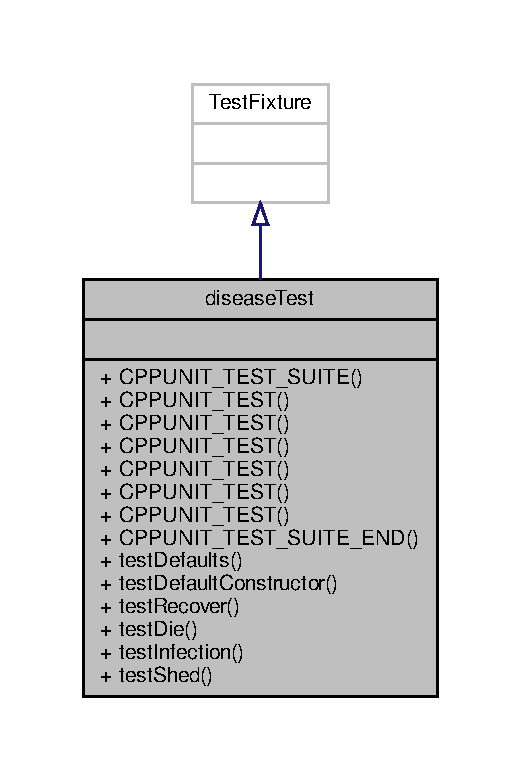
\includegraphics[width=250pt]{classdiseaseTest__inherit__graph}
\end{center}
\end{figure}


Collaboration diagram for disease\+Test\+:\nopagebreak
\begin{figure}[H]
\begin{center}
\leavevmode
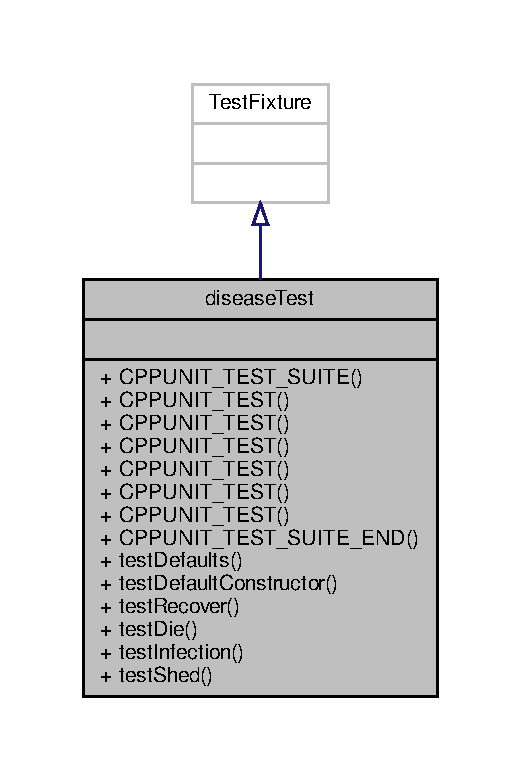
\includegraphics[width=250pt]{classdiseaseTest__coll__graph}
\end{center}
\end{figure}
\subsection*{Public Member Functions}
\begin{DoxyCompactItemize}
\item 
\mbox{\Hypertarget{classdiseaseTest_af7f1b00d3ae875d3314e3c5c6020212a}\label{classdiseaseTest_af7f1b00d3ae875d3314e3c5c6020212a}} 
\mbox{\hyperlink{classdiseaseTest_af7f1b00d3ae875d3314e3c5c6020212a}{C\+P\+P\+U\+N\+I\+T\+\_\+\+T\+E\+S\+T\+\_\+\+S\+U\+I\+TE}} (\mbox{\hyperlink{classdiseaseTest}{disease\+Test}})
\begin{DoxyCompactList}\small\item\em automatically create a test suite to add tests to \end{DoxyCompactList}\item 
\mbox{\Hypertarget{classdiseaseTest_aa0f6c0aa41fae9d84b8d36f099e66153}\label{classdiseaseTest_aa0f6c0aa41fae9d84b8d36f099e66153}} 
\mbox{\hyperlink{classdiseaseTest_aa0f6c0aa41fae9d84b8d36f099e66153}{C\+P\+P\+U\+N\+I\+T\+\_\+\+T\+E\+ST}} (\mbox{\hyperlink{classdiseaseTest_a76ac8d52f421ccb010d5be72228fe613}{test\+Defaults}})
\begin{DoxyCompactList}\small\item\em check defaults \end{DoxyCompactList}\item 
\mbox{\Hypertarget{classdiseaseTest_a9c6fb710bc0f891eb89c2b47b234e902}\label{classdiseaseTest_a9c6fb710bc0f891eb89c2b47b234e902}} 
\mbox{\hyperlink{classdiseaseTest_a9c6fb710bc0f891eb89c2b47b234e902}{C\+P\+P\+U\+N\+I\+T\+\_\+\+T\+E\+ST}} (\mbox{\hyperlink{classdiseaseTest_a1559f0bcf9c829f890b891ded00c746f}{test\+Default\+Constructor}})
\begin{DoxyCompactList}\small\item\em test out constructor \end{DoxyCompactList}\item 
\mbox{\Hypertarget{classdiseaseTest_aab2e2a22338a2752edf1a41e869befdf}\label{classdiseaseTest_aab2e2a22338a2752edf1a41e869befdf}} 
\mbox{\hyperlink{classdiseaseTest_aab2e2a22338a2752edf1a41e869befdf}{C\+P\+P\+U\+N\+I\+T\+\_\+\+T\+E\+ST}} (\mbox{\hyperlink{classdiseaseTest_af072ce110dc0cb4e4dfd7938e03e01f4}{test\+Recover}})
\begin{DoxyCompactList}\small\item\em test recovery from disease \end{DoxyCompactList}\item 
\mbox{\Hypertarget{classdiseaseTest_aae0e823489f65dce639bc1fec9105d25}\label{classdiseaseTest_aae0e823489f65dce639bc1fec9105d25}} 
\mbox{\hyperlink{classdiseaseTest_aae0e823489f65dce639bc1fec9105d25}{C\+P\+P\+U\+N\+I\+T\+\_\+\+T\+E\+ST}} (\mbox{\hyperlink{classdiseaseTest_a703842c90288f26dbe79fec811b7e214}{test\+Die}})
\begin{DoxyCompactList}\small\item\em test out the death function \end{DoxyCompactList}\item 
\mbox{\Hypertarget{classdiseaseTest_af0c1b19108a6cc01a63fb65dda68da43}\label{classdiseaseTest_af0c1b19108a6cc01a63fb65dda68da43}} 
\mbox{\hyperlink{classdiseaseTest_af0c1b19108a6cc01a63fb65dda68da43}{C\+P\+P\+U\+N\+I\+T\+\_\+\+T\+E\+ST}} (\mbox{\hyperlink{classdiseaseTest_ac6ddc9154b76e19798cd72c144d67c53}{test\+Infection}})
\begin{DoxyCompactList}\small\item\em check how infection is acquired \end{DoxyCompactList}\item 
\mbox{\Hypertarget{classdiseaseTest_a8353330ff74b1589854261529a113c9b}\label{classdiseaseTest_a8353330ff74b1589854261529a113c9b}} 
\mbox{\hyperlink{classdiseaseTest_a8353330ff74b1589854261529a113c9b}{C\+P\+P\+U\+N\+I\+T\+\_\+\+T\+E\+ST}} (\mbox{\hyperlink{classdiseaseTest_aec9719173d92e888f32ada40f567467a}{test\+Shed}})
\begin{DoxyCompactList}\small\item\em test contamination shedding \end{DoxyCompactList}\item 
\mbox{\Hypertarget{classdiseaseTest_a1940da2c66267bf403173256c7f112aa}\label{classdiseaseTest_a1940da2c66267bf403173256c7f112aa}} 
\mbox{\hyperlink{classdiseaseTest_a1940da2c66267bf403173256c7f112aa}{C\+P\+P\+U\+N\+I\+T\+\_\+\+T\+E\+S\+T\+\_\+\+S\+U\+I\+T\+E\+\_\+\+E\+ND}} ()
\begin{DoxyCompactList}\small\item\em end test suite \end{DoxyCompactList}\item 
\mbox{\Hypertarget{classdiseaseTest_a76ac8d52f421ccb010d5be72228fe613}\label{classdiseaseTest_a76ac8d52f421ccb010d5be72228fe613}} 
void \mbox{\hyperlink{classdiseaseTest_a76ac8d52f421ccb010d5be72228fe613}{test\+Defaults}} ()
\begin{DoxyCompactList}\small\item\em since this is a static class defaults should be as in disease.\+cpp \end{DoxyCompactList}\item 
\mbox{\Hypertarget{classdiseaseTest_a1559f0bcf9c829f890b891ded00c746f}\label{classdiseaseTest_a1559f0bcf9c829f890b891ded00c746f}} 
void \mbox{\hyperlink{classdiseaseTest_a1559f0bcf9c829f890b891ded00c746f}{test\+Default\+Constructor}} ()
\begin{DoxyCompactList}\small\item\em by defining an object values are set by teh constructor rater than defaults \end{DoxyCompactList}\item 
void \mbox{\hyperlink{classdiseaseTest_af072ce110dc0cb4e4dfd7938e03e01f4}{test\+Recover}} ()
\begin{DoxyCompactList}\small\item\em given two identical random sequences, recovery should be the same \end{DoxyCompactList}\item 
\mbox{\Hypertarget{classdiseaseTest_a703842c90288f26dbe79fec811b7e214}\label{classdiseaseTest_a703842c90288f26dbe79fec811b7e214}} 
void \mbox{\hyperlink{classdiseaseTest_a703842c90288f26dbe79fec811b7e214}{test\+Die}} ()
\begin{DoxyCompactList}\small\item\em the death function looks just like the recovery function so test in the same way \end{DoxyCompactList}\item 
void \mbox{\hyperlink{classdiseaseTest_ac6ddc9154b76e19798cd72c144d67c53}{test\+Infection}} ()
\begin{DoxyCompactList}\small\item\em again use two identical random sequences to check infection \end{DoxyCompactList}\item 
\mbox{\Hypertarget{classdiseaseTest_aec9719173d92e888f32ada40f567467a}\label{classdiseaseTest_aec9719173d92e888f32ada40f567467a}} 
void \mbox{\hyperlink{classdiseaseTest_aec9719173d92e888f32ada40f567467a}{test\+Shed}} ()
\begin{DoxyCompactList}\small\item\em Check infection shedding is independent of timestep unit also. \end{DoxyCompactList}\end{DoxyCompactItemize}


\subsection{Detailed Description}
test the disease static classs 

\subsection{Member Function Documentation}
\mbox{\Hypertarget{classdiseaseTest_ac6ddc9154b76e19798cd72c144d67c53}\label{classdiseaseTest_ac6ddc9154b76e19798cd72c144d67c53}} 
\index{disease\+Test@{disease\+Test}!test\+Infection@{test\+Infection}}
\index{test\+Infection@{test\+Infection}!disease\+Test@{disease\+Test}}
\subsubsection{\texorpdfstring{test\+Infection()}{testInfection()}}
{\footnotesize\ttfamily void disease\+Test\+::test\+Infection (\begin{DoxyParamCaption}{ }\end{DoxyParamCaption})\hspace{0.3cm}{\ttfamily [inline]}}



again use two identical random sequences to check infection 

this should just depend on the contamination level and the rate per hour. \mbox{\Hypertarget{classdiseaseTest_af072ce110dc0cb4e4dfd7938e03e01f4}\label{classdiseaseTest_af072ce110dc0cb4e4dfd7938e03e01f4}} 
\index{disease\+Test@{disease\+Test}!test\+Recover@{test\+Recover}}
\index{test\+Recover@{test\+Recover}!disease\+Test@{disease\+Test}}
\subsubsection{\texorpdfstring{test\+Recover()}{testRecover()}}
{\footnotesize\ttfamily void disease\+Test\+::test\+Recover (\begin{DoxyParamCaption}{ }\end{DoxyParamCaption})\hspace{0.3cm}{\ttfamily [inline]}}



given two identical random sequences, recovery should be the same 

explcitly check that the function call to disease matches the function content. Also make ~\newline
sure that the timestepping guarantees the same rate per unit time independentof time unit 

The documentation for this class was generated from the following file\+:\begin{DoxyCompactItemize}
\item 
\mbox{\hyperlink{diseasetest_8h}{diseasetest.\+h}}\end{DoxyCompactItemize}

\hypertarget{classmodelFactoryTest}{}\section{model\+Factory\+Test Class Reference}
\label{classmodelFactoryTest}\index{model\+Factory\+Test@{model\+Factory\+Test}}


test out the model\+Factory class  




{\ttfamily \#include $<$modelfactorytest.\+h$>$}



Inheritance diagram for model\+Factory\+Test\+:\nopagebreak
\begin{figure}[H]
\begin{center}
\leavevmode
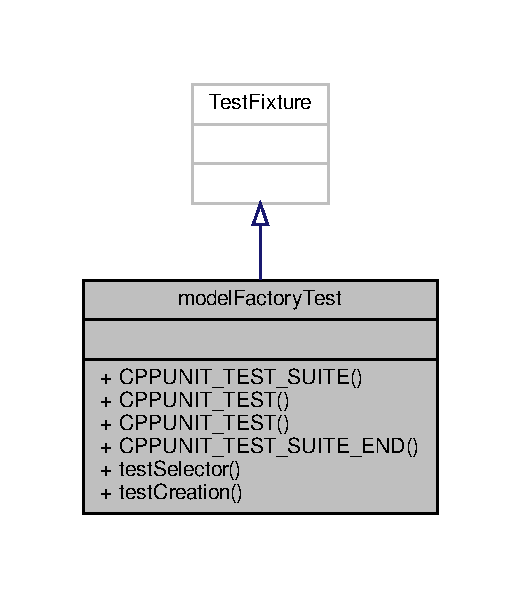
\includegraphics[width=250pt]{classmodelFactoryTest__inherit__graph}
\end{center}
\end{figure}


Collaboration diagram for model\+Factory\+Test\+:\nopagebreak
\begin{figure}[H]
\begin{center}
\leavevmode
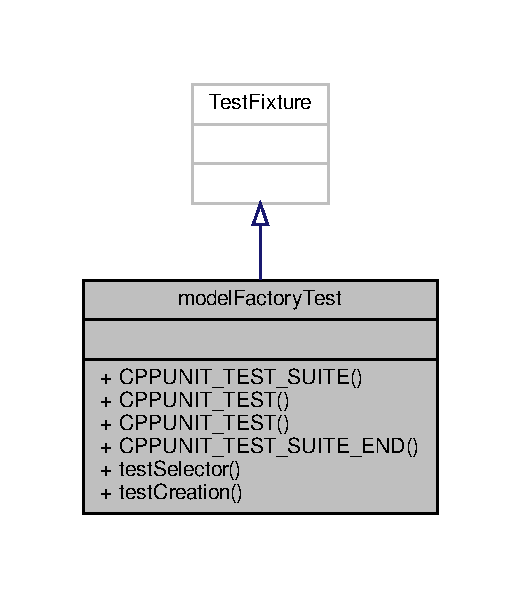
\includegraphics[width=250pt]{classmodelFactoryTest__coll__graph}
\end{center}
\end{figure}
\subsection*{Public Member Functions}
\begin{DoxyCompactItemize}
\item 
\mbox{\Hypertarget{classmodelFactoryTest_a20b209282561b641257928824314a49c}\label{classmodelFactoryTest_a20b209282561b641257928824314a49c}} 
\mbox{\hyperlink{classmodelFactoryTest_a20b209282561b641257928824314a49c}{C\+P\+P\+U\+N\+I\+T\+\_\+\+T\+E\+S\+T\+\_\+\+S\+U\+I\+TE}} (\mbox{\hyperlink{classmodelFactoryTest}{model\+Factory\+Test}})
\begin{DoxyCompactList}\small\item\em automatically create a test suite to add tests to \end{DoxyCompactList}\item 
\mbox{\Hypertarget{classmodelFactoryTest_a52899c75fe7f21fd6a1c96151302bb5a}\label{classmodelFactoryTest_a52899c75fe7f21fd6a1c96151302bb5a}} 
\mbox{\hyperlink{classmodelFactoryTest_a52899c75fe7f21fd6a1c96151302bb5a}{C\+P\+P\+U\+N\+I\+T\+\_\+\+T\+E\+ST}} (\mbox{\hyperlink{classmodelFactoryTest_ae0327f9c7d653c9a4864122a3f088118}{test\+Selector}})
\begin{DoxyCompactList}\small\item\em test the factory selector method \end{DoxyCompactList}\item 
\mbox{\Hypertarget{classmodelFactoryTest_a46a5eadbc8f9d03e0c6d5334ee687d49}\label{classmodelFactoryTest_a46a5eadbc8f9d03e0c6d5334ee687d49}} 
\mbox{\hyperlink{classmodelFactoryTest_a46a5eadbc8f9d03e0c6d5334ee687d49}{C\+P\+P\+U\+N\+I\+T\+\_\+\+T\+E\+ST}} (\mbox{\hyperlink{classmodelFactoryTest_a1bea8789a99ca88af5942eaf6c3fa687}{test\+Creation}})
\begin{DoxyCompactList}\small\item\em check agent and place creation \end{DoxyCompactList}\item 
\mbox{\Hypertarget{classmodelFactoryTest_a8f11a0a4ce2d23277167233305b1040e}\label{classmodelFactoryTest_a8f11a0a4ce2d23277167233305b1040e}} 
\mbox{\hyperlink{classmodelFactoryTest_a8f11a0a4ce2d23277167233305b1040e}{C\+P\+P\+U\+N\+I\+T\+\_\+\+T\+E\+S\+T\+\_\+\+S\+U\+I\+T\+E\+\_\+\+E\+ND}} ()
\begin{DoxyCompactList}\small\item\em end the test suite \end{DoxyCompactList}\item 
\mbox{\Hypertarget{classmodelFactoryTest_ae0327f9c7d653c9a4864122a3f088118}\label{classmodelFactoryTest_ae0327f9c7d653c9a4864122a3f088118}} 
void \mbox{\hyperlink{classmodelFactoryTest_ae0327f9c7d653c9a4864122a3f088118}{test\+Selector}} ()
\begin{DoxyCompactList}\small\item\em make sure the selector works \end{DoxyCompactList}\item 
\mbox{\Hypertarget{classmodelFactoryTest_a1bea8789a99ca88af5942eaf6c3fa687}\label{classmodelFactoryTest_a1bea8789a99ca88af5942eaf6c3fa687}} 
void \mbox{\hyperlink{classmodelFactoryTest_a1bea8789a99ca88af5942eaf6c3fa687}{test\+Creation}} ()
\begin{DoxyCompactList}\small\item\em check the creation of agents and places looks OK \end{DoxyCompactList}\end{DoxyCompactItemize}


\subsection{Detailed Description}
test out the model\+Factory class 

The documentation for this class was generated from the following file\+:\begin{DoxyCompactItemize}
\item 
\mbox{\hyperlink{modelfactorytest_8h}{modelfactorytest.\+h}}\end{DoxyCompactItemize}

\hypertarget{classmodelTest}{}\section{model\+Test Class Reference}
\label{classmodelTest}\index{model\+Test@{model\+Test}}


test out the model class  




{\ttfamily \#include $<$modeltest.\+h$>$}



Inheritance diagram for model\+Test\+:\nopagebreak
\begin{figure}[H]
\begin{center}
\leavevmode
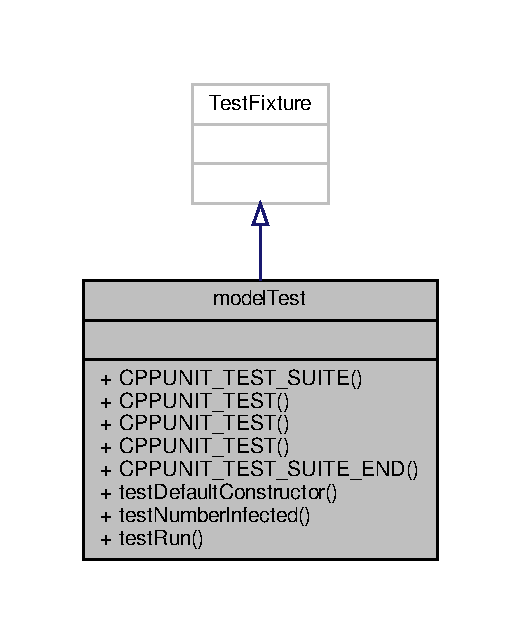
\includegraphics[width=250pt]{classmodelTest__inherit__graph}
\end{center}
\end{figure}


Collaboration diagram for model\+Test\+:\nopagebreak
\begin{figure}[H]
\begin{center}
\leavevmode
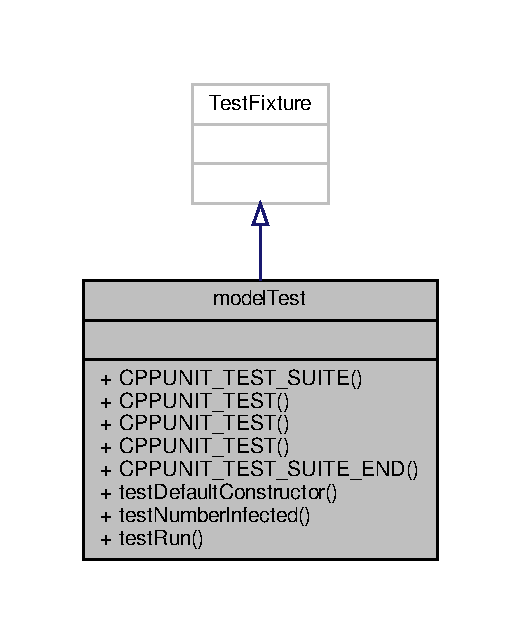
\includegraphics[width=250pt]{classmodelTest__coll__graph}
\end{center}
\end{figure}
\subsection*{Public Member Functions}
\begin{DoxyCompactItemize}
\item 
\mbox{\Hypertarget{classmodelTest_afd8cee8035be15212f9236c2cf5b1bde}\label{classmodelTest_afd8cee8035be15212f9236c2cf5b1bde}} 
\mbox{\hyperlink{classmodelTest_afd8cee8035be15212f9236c2cf5b1bde}{C\+P\+P\+U\+N\+I\+T\+\_\+\+T\+E\+S\+T\+\_\+\+S\+U\+I\+TE}} (\mbox{\hyperlink{classmodelTest}{model\+Test}})
\begin{DoxyCompactList}\small\item\em automatically create a test suite to add tests to \end{DoxyCompactList}\item 
\mbox{\Hypertarget{classmodelTest_aa1691735f57c35d37d358ef56dfdc97e}\label{classmodelTest_aa1691735f57c35d37d358ef56dfdc97e}} 
\mbox{\hyperlink{classmodelTest_aa1691735f57c35d37d358ef56dfdc97e}{C\+P\+P\+U\+N\+I\+T\+\_\+\+T\+E\+ST}} (\mbox{\hyperlink{classmodelTest_a1ec93676ece4bbb6f98cf65340472939}{test\+Default\+Constructor}})
\begin{DoxyCompactList}\small\item\em test the default constructor \end{DoxyCompactList}\item 
\mbox{\Hypertarget{classmodelTest_ab189eb8152f72c53c6437d9e54e5a374}\label{classmodelTest_ab189eb8152f72c53c6437d9e54e5a374}} 
\mbox{\hyperlink{classmodelTest_ab189eb8152f72c53c6437d9e54e5a374}{C\+P\+P\+U\+N\+I\+T\+\_\+\+T\+E\+ST}} (\mbox{\hyperlink{classmodelTest_ab7a0f9094aaab12eadc0fedbb57505e8}{test\+Number\+Infected}})
\begin{DoxyCompactList}\small\item\em test the default constructor \end{DoxyCompactList}\item 
\mbox{\Hypertarget{classmodelTest_a3596a54ba85399f6d293fb928041f9a5}\label{classmodelTest_a3596a54ba85399f6d293fb928041f9a5}} 
\mbox{\hyperlink{classmodelTest_a3596a54ba85399f6d293fb928041f9a5}{C\+P\+P\+U\+N\+I\+T\+\_\+\+T\+E\+ST}} (\mbox{\hyperlink{classmodelTest_a18ccf91ea0223e52d439fa267665d718}{test\+Run}})
\begin{DoxyCompactList}\small\item\em test run \end{DoxyCompactList}\item 
\mbox{\Hypertarget{classmodelTest_a704621b184dbdb454d4cf0f90d4d210c}\label{classmodelTest_a704621b184dbdb454d4cf0f90d4d210c}} 
\mbox{\hyperlink{classmodelTest_a704621b184dbdb454d4cf0f90d4d210c}{C\+P\+P\+U\+N\+I\+T\+\_\+\+T\+E\+S\+T\+\_\+\+S\+U\+I\+T\+E\+\_\+\+E\+ND}} ()
\begin{DoxyCompactList}\small\item\em end the test suite \end{DoxyCompactList}\item 
\mbox{\Hypertarget{classmodelTest_a1ec93676ece4bbb6f98cf65340472939}\label{classmodelTest_a1ec93676ece4bbb6f98cf65340472939}} 
void \mbox{\hyperlink{classmodelTest_a1ec93676ece4bbb6f98cf65340472939}{test\+Default\+Constructor}} ()
\begin{DoxyCompactList}\small\item\em make sure results from constructor are as expected for simple mobile model \end{DoxyCompactList}\item 
void \mbox{\hyperlink{classmodelTest_ab7a0f9094aaab12eadc0fedbb57505e8}{test\+Number\+Infected}} ()
\begin{DoxyCompactList}\small\item\em in the simple disease the initial number infected should not be able to exceed the agent number \end{DoxyCompactList}\item 
void \mbox{\hyperlink{classmodelTest_a18ccf91ea0223e52d439fa267665d718}{test\+Run}} ()
\begin{DoxyCompactList}\small\item\em try stepping the model forward and check output \end{DoxyCompactList}\end{DoxyCompactItemize}


\subsection{Detailed Description}
test out the model class 

\subsection{Member Function Documentation}
\mbox{\Hypertarget{classmodelTest_ab7a0f9094aaab12eadc0fedbb57505e8}\label{classmodelTest_ab7a0f9094aaab12eadc0fedbb57505e8}} 
\index{model\+Test@{model\+Test}!test\+Number\+Infected@{test\+Number\+Infected}}
\index{test\+Number\+Infected@{test\+Number\+Infected}!model\+Test@{model\+Test}}
\subsubsection{\texorpdfstring{test\+Number\+Infected()}{testNumberInfected()}}
{\footnotesize\ttfamily void model\+Test\+::test\+Number\+Infected (\begin{DoxyParamCaption}{ }\end{DoxyParamCaption})\hspace{0.3cm}{\ttfamily [inline]}}



in the simple disease the initial number infected should not be able to exceed the agent number 

If more than the number of agents is requested, then the code is expected to max. this out~\newline
as the total number of agents initially present \mbox{\Hypertarget{classmodelTest_a18ccf91ea0223e52d439fa267665d718}\label{classmodelTest_a18ccf91ea0223e52d439fa267665d718}} 
\index{model\+Test@{model\+Test}!test\+Run@{test\+Run}}
\index{test\+Run@{test\+Run}!model\+Test@{model\+Test}}
\subsubsection{\texorpdfstring{test\+Run()}{testRun()}}
{\footnotesize\ttfamily void model\+Test\+::test\+Run (\begin{DoxyParamCaption}{ }\end{DoxyParamCaption})\hspace{0.3cm}{\ttfamily [inline]}}



try stepping the model forward and check output 

if the number of omp threads is not set this can produce crashes or unpredictable results... 

The documentation for this class was generated from the following file\+:\begin{DoxyCompactItemize}
\item 
\mbox{\hyperlink{modeltest_8h}{modeltest.\+h}}\end{DoxyCompactItemize}

\hypertarget{classMyCustomProgressTestListener}{}\section{My\+Custom\+Progress\+Test\+Listener Class Reference}
\label{classMyCustomProgressTestListener}\index{My\+Custom\+Progress\+Test\+Listener@{My\+Custom\+Progress\+Test\+Listener}}


Report the start of each test.  




Inheritance diagram for My\+Custom\+Progress\+Test\+Listener\+:\nopagebreak
\begin{figure}[H]
\begin{center}
\leavevmode
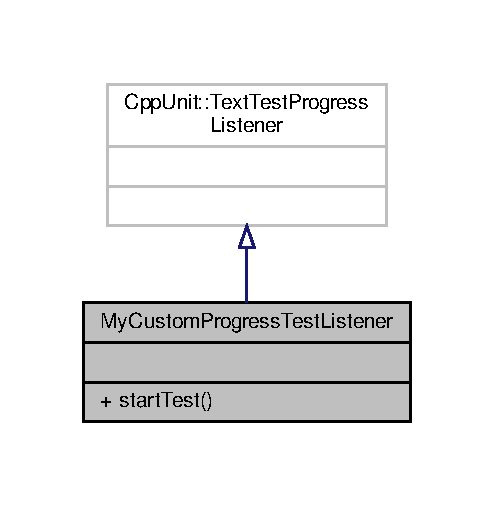
\includegraphics[width=237pt]{classMyCustomProgressTestListener__inherit__graph}
\end{center}
\end{figure}


Collaboration diagram for My\+Custom\+Progress\+Test\+Listener\+:\nopagebreak
\begin{figure}[H]
\begin{center}
\leavevmode
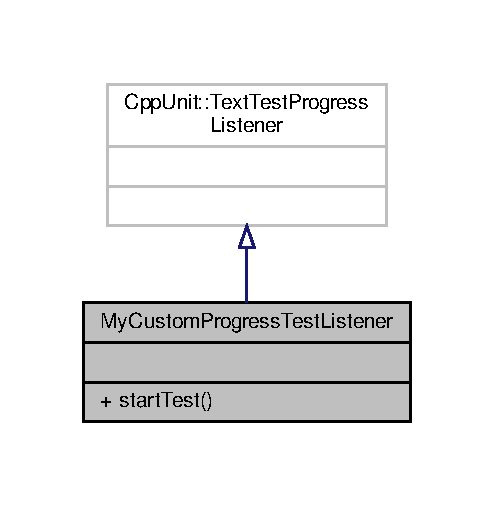
\includegraphics[width=237pt]{classMyCustomProgressTestListener__coll__graph}
\end{center}
\end{figure}
\subsection*{Public Member Functions}
\begin{DoxyCompactItemize}
\item 
virtual void \mbox{\hyperlink{classMyCustomProgressTestListener_a798f9c66a689cbe41701b582b9033892}{start\+Test}} (Cpp\+Unit\+::\+Test $\ast$test)
\begin{DoxyCompactList}\small\item\em define the message to be printed when each test starts \end{DoxyCompactList}\end{DoxyCompactItemize}


\subsection{Detailed Description}
Report the start of each test. 

Define a class that will print a message to stdout as each test is started. ~\newline
An instance of this class gets added to the Cpp\+Unit\+::\+Text\+Ui\+::\+Test\+Runner that runs the test suites 

\subsection{Member Function Documentation}
\mbox{\Hypertarget{classMyCustomProgressTestListener_a798f9c66a689cbe41701b582b9033892}\label{classMyCustomProgressTestListener_a798f9c66a689cbe41701b582b9033892}} 
\index{My\+Custom\+Progress\+Test\+Listener@{My\+Custom\+Progress\+Test\+Listener}!start\+Test@{start\+Test}}
\index{start\+Test@{start\+Test}!My\+Custom\+Progress\+Test\+Listener@{My\+Custom\+Progress\+Test\+Listener}}
\subsubsection{\texorpdfstring{start\+Test()}{startTest()}}
{\footnotesize\ttfamily virtual void My\+Custom\+Progress\+Test\+Listener\+::start\+Test (\begin{DoxyParamCaption}\item[{Cpp\+Unit\+::\+Test $\ast$}]{test }\end{DoxyParamCaption})\hspace{0.3cm}{\ttfamily [inline]}, {\ttfamily [virtual]}}



define the message to be printed when each test starts 

The name of the current running test is extracted using test-\/$>$get\+Name() 
\begin{DoxyParams}{Parameters}
{\em test} & a pointer to a Cpp\+Unit\+::test object \\
\hline
\end{DoxyParams}


The documentation for this class was generated from the following file\+:\begin{DoxyCompactItemize}
\item 
\mbox{\hyperlink{testing_8cpp}{testing.\+cpp}}\end{DoxyCompactItemize}

\hypertarget{classparameterTest}{}\section{parameter\+Test Class Reference}
\label{classparameterTest}\index{parameter\+Test@{parameter\+Test}}


Check parameter defaults are as expected.  




{\ttfamily \#include $<$parametertest.\+h$>$}



Inheritance diagram for parameter\+Test\+:\nopagebreak
\begin{figure}[H]
\begin{center}
\leavevmode
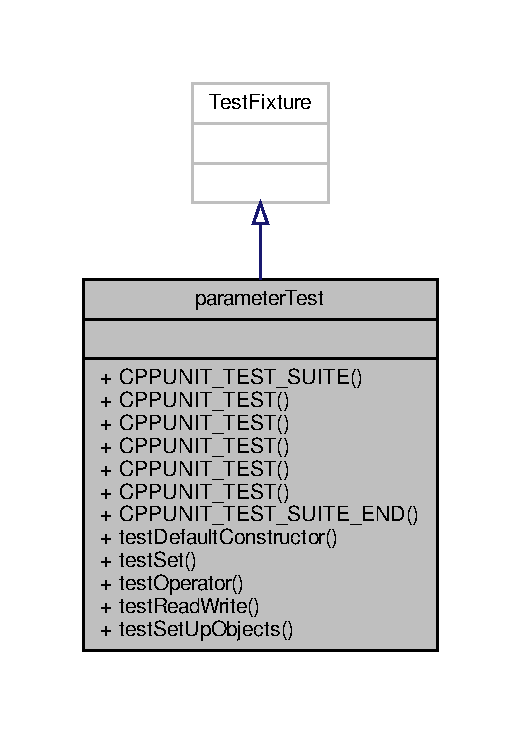
\includegraphics[width=250pt]{classparameterTest__inherit__graph}
\end{center}
\end{figure}


Collaboration diagram for parameter\+Test\+:\nopagebreak
\begin{figure}[H]
\begin{center}
\leavevmode
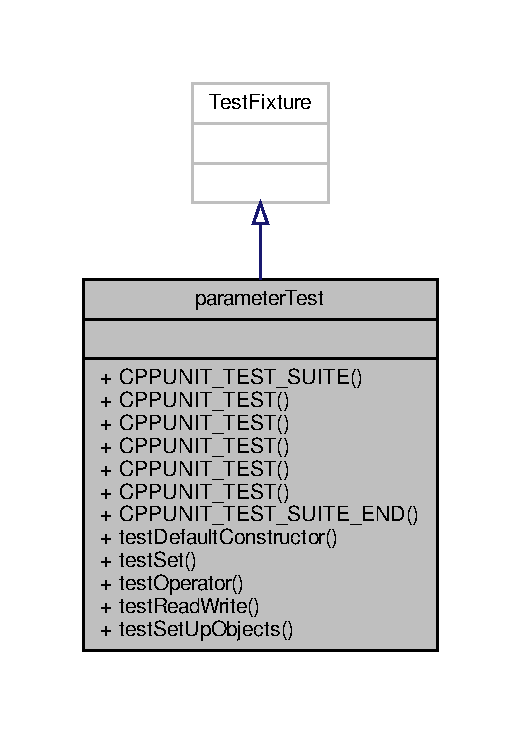
\includegraphics[width=250pt]{classparameterTest__coll__graph}
\end{center}
\end{figure}
\subsection*{Public Member Functions}
\begin{DoxyCompactItemize}
\item 
\mbox{\Hypertarget{classparameterTest_a10e241ba4df333675089b47d53738345}\label{classparameterTest_a10e241ba4df333675089b47d53738345}} 
\mbox{\hyperlink{classparameterTest_a10e241ba4df333675089b47d53738345}{C\+P\+P\+U\+N\+I\+T\+\_\+\+T\+E\+S\+T\+\_\+\+S\+U\+I\+TE}} (\mbox{\hyperlink{classparameterTest}{parameter\+Test}})
\begin{DoxyCompactList}\small\item\em automatically create a test suite to add tests to \end{DoxyCompactList}\item 
\mbox{\Hypertarget{classparameterTest_aae669ac4378b05b1f3a46973382cdac8}\label{classparameterTest_aae669ac4378b05b1f3a46973382cdac8}} 
\mbox{\hyperlink{classparameterTest_aae669ac4378b05b1f3a46973382cdac8}{C\+P\+P\+U\+N\+I\+T\+\_\+\+T\+E\+ST}} (\mbox{\hyperlink{classparameterTest_a80bc49c4dafb3b6ae5c7e561b5711583}{test\+Default\+Constructor}})
\begin{DoxyCompactList}\small\item\em constructor shoudl set defaults for all parameters \end{DoxyCompactList}\item 
\mbox{\Hypertarget{classparameterTest_a21c4cabbb339e5d6af1e69628b57596f}\label{classparameterTest_a21c4cabbb339e5d6af1e69628b57596f}} 
\mbox{\hyperlink{classparameterTest_a21c4cabbb339e5d6af1e69628b57596f}{C\+P\+P\+U\+N\+I\+T\+\_\+\+T\+E\+ST}} (\mbox{\hyperlink{classparameterTest_ae8748da779947e5ddac496a38e1b07b8}{test\+Set}})
\begin{DoxyCompactList}\small\item\em parameters should be settable \end{DoxyCompactList}\item 
\mbox{\Hypertarget{classparameterTest_a409fee522f591e3ea4a24bc4d4f6931d}\label{classparameterTest_a409fee522f591e3ea4a24bc4d4f6931d}} 
\mbox{\hyperlink{classparameterTest_a409fee522f591e3ea4a24bc4d4f6931d}{C\+P\+P\+U\+N\+I\+T\+\_\+\+T\+E\+ST}} (\mbox{\hyperlink{classparameterTest_a099ef3c9d0a74ada96f9dd8bd4c168e6}{test\+Operator}})
\begin{DoxyCompactList}\small\item\em operator () returns string value \end{DoxyCompactList}\item 
\mbox{\Hypertarget{classparameterTest_a02fb4f6ddf3874f79f120abfb0d56c82}\label{classparameterTest_a02fb4f6ddf3874f79f120abfb0d56c82}} 
\mbox{\hyperlink{classparameterTest_a02fb4f6ddf3874f79f120abfb0d56c82}{C\+P\+P\+U\+N\+I\+T\+\_\+\+T\+E\+ST}} (\mbox{\hyperlink{classparameterTest_a73ffa897b723095fdb3f06cc309575d6}{test\+Read\+Write}})
\begin{DoxyCompactList}\small\item\em read and write parameter settings \end{DoxyCompactList}\item 
\mbox{\Hypertarget{classparameterTest_a2346e04084e15821605e7da477af0fb3}\label{classparameterTest_a2346e04084e15821605e7da477af0fb3}} 
\mbox{\hyperlink{classparameterTest_a2346e04084e15821605e7da477af0fb3}{C\+P\+P\+U\+N\+I\+T\+\_\+\+T\+E\+ST}} (\mbox{\hyperlink{classparameterTest_aeb4d3a1620defdc974a9b925f4c1cd9f}{test\+Set\+Up\+Objects}})
\begin{DoxyCompactList}\small\item\em Test settings in other objects. \end{DoxyCompactList}\item 
\mbox{\Hypertarget{classparameterTest_a051c68e665c44e09d98bffd0b6c7b78a}\label{classparameterTest_a051c68e665c44e09d98bffd0b6c7b78a}} 
\mbox{\hyperlink{classparameterTest_a051c68e665c44e09d98bffd0b6c7b78a}{C\+P\+P\+U\+N\+I\+T\+\_\+\+T\+E\+S\+T\+\_\+\+S\+U\+I\+T\+E\+\_\+\+E\+ND}} ()
\begin{DoxyCompactList}\small\item\em End test suite. \end{DoxyCompactList}\item 
void \mbox{\hyperlink{classparameterTest_a80bc49c4dafb3b6ae5c7e561b5711583}{test\+Default\+Constructor}} ()
\begin{DoxyCompactList}\small\item\em The default constructor calls the setdefaults function. \end{DoxyCompactList}\item 
void \mbox{\hyperlink{classparameterTest_ae8748da779947e5ddac496a38e1b07b8}{test\+Set}} ()
\begin{DoxyCompactList}\small\item\em Check settings of individual parameters works. \end{DoxyCompactList}\item 
void \mbox{\hyperlink{classparameterTest_a099ef3c9d0a74ada96f9dd8bd4c168e6}{test\+Operator}} ()
\begin{DoxyCompactList}\small\item\em The operator () should return the string value corresponding to any parameter. \end{DoxyCompactList}\item 
void \mbox{\hyperlink{classparameterTest_a73ffa897b723095fdb3f06cc309575d6}{test\+Read\+Write}} ()
\begin{DoxyCompactList}\small\item\em Check input and output of parameter settings. \end{DoxyCompactList}\item 
void \mbox{\hyperlink{classparameterTest_aeb4d3a1620defdc974a9b925f4c1cd9f}{test\+Set\+Up\+Objects}} ()
\begin{DoxyCompactList}\small\item\em Check some of the other classes are getting the right input from the parameter\+Settings objects. \end{DoxyCompactList}\end{DoxyCompactItemize}


\subsection{Detailed Description}
Check parameter defaults are as expected. 

Setting of parameters and ability to read from and write out to a file are checked. ~\newline
The input file is called test\+Parameter\+File, and the output Run\+Parameters.~\newline
Text showing parameter settings is also displayed on stdout. 

\subsection{Member Function Documentation}
\mbox{\Hypertarget{classparameterTest_a80bc49c4dafb3b6ae5c7e561b5711583}\label{classparameterTest_a80bc49c4dafb3b6ae5c7e561b5711583}} 
\index{parameter\+Test@{parameter\+Test}!test\+Default\+Constructor@{test\+Default\+Constructor}}
\index{test\+Default\+Constructor@{test\+Default\+Constructor}!parameter\+Test@{parameter\+Test}}
\subsubsection{\texorpdfstring{test\+Default\+Constructor()}{testDefaultConstructor()}}
{\footnotesize\ttfamily void parameter\+Test\+::test\+Default\+Constructor (\begin{DoxyParamCaption}{ }\end{DoxyParamCaption})\hspace{0.3cm}{\ttfamily [inline]}}



The default constructor calls the setdefaults function. 

The values here are copied directly from that function. Also tests that the get$<$$>$ methods~\newline
correctly retrieve parmeters of the right datatype \mbox{\Hypertarget{classparameterTest_a099ef3c9d0a74ada96f9dd8bd4c168e6}\label{classparameterTest_a099ef3c9d0a74ada96f9dd8bd4c168e6}} 
\index{parameter\+Test@{parameter\+Test}!test\+Operator@{test\+Operator}}
\index{test\+Operator@{test\+Operator}!parameter\+Test@{parameter\+Test}}
\subsubsection{\texorpdfstring{test\+Operator()}{testOperator()}}
{\footnotesize\ttfamily void parameter\+Test\+::test\+Operator (\begin{DoxyParamCaption}{ }\end{DoxyParamCaption})\hspace{0.3cm}{\ttfamily [inline]}}



The operator () should return the string value corresponding to any parameter. 

check strings are as expected from defaults \mbox{\Hypertarget{classparameterTest_a73ffa897b723095fdb3f06cc309575d6}\label{classparameterTest_a73ffa897b723095fdb3f06cc309575d6}} 
\index{parameter\+Test@{parameter\+Test}!test\+Read\+Write@{test\+Read\+Write}}
\index{test\+Read\+Write@{test\+Read\+Write}!parameter\+Test@{parameter\+Test}}
\subsubsection{\texorpdfstring{test\+Read\+Write()}{testReadWrite()}}
{\footnotesize\ttfamily void parameter\+Test\+::test\+Read\+Write (\begin{DoxyParamCaption}{ }\end{DoxyParamCaption})\hspace{0.3cm}{\ttfamily [inline]}}



Check input and output of parameter settings. 

The default output file is called Run\+Parameters -\/ here just the path is set to the current directory.~\newline
 A few of the values from the input file test\+Parameter\+File are checked where they differ from defaults \mbox{\Hypertarget{classparameterTest_ae8748da779947e5ddac496a38e1b07b8}\label{classparameterTest_ae8748da779947e5ddac496a38e1b07b8}} 
\index{parameter\+Test@{parameter\+Test}!test\+Set@{test\+Set}}
\index{test\+Set@{test\+Set}!parameter\+Test@{parameter\+Test}}
\subsubsection{\texorpdfstring{test\+Set()}{testSet()}}
{\footnotesize\ttfamily void parameter\+Test\+::test\+Set (\begin{DoxyParamCaption}{ }\end{DoxyParamCaption})\hspace{0.3cm}{\ttfamily [inline]}}



Check settings of individual parameters works. 

make sure that the string values in set get retrieved as correct data values \mbox{\Hypertarget{classparameterTest_aeb4d3a1620defdc974a9b925f4c1cd9f}\label{classparameterTest_aeb4d3a1620defdc974a9b925f4c1cd9f}} 
\index{parameter\+Test@{parameter\+Test}!test\+Set\+Up\+Objects@{test\+Set\+Up\+Objects}}
\index{test\+Set\+Up\+Objects@{test\+Set\+Up\+Objects}!parameter\+Test@{parameter\+Test}}
\subsubsection{\texorpdfstring{test\+Set\+Up\+Objects()}{testSetUpObjects()}}
{\footnotesize\ttfamily void parameter\+Test\+::test\+Set\+Up\+Objects (\begin{DoxyParamCaption}{ }\end{DoxyParamCaption})\hspace{0.3cm}{\ttfamily [inline]}}



Check some of the other classes are getting the right input from the parameter\+Settings objects. 

In this case the static time\+Step and disease, as well as the places 

The documentation for this class was generated from the following file\+:\begin{DoxyCompactItemize}
\item 
\mbox{\hyperlink{parametertest_8h}{parametertest.\+h}}\end{DoxyCompactItemize}

\hypertarget{classplaceTest}{}\section{place\+Test Class Reference}
\label{classplaceTest}\index{place\+Test@{place\+Test}}


Check places for contamination levels and agent occupancy.  




{\ttfamily \#include $<$placetest.\+h$>$}



Inheritance diagram for place\+Test\+:\nopagebreak
\begin{figure}[H]
\begin{center}
\leavevmode
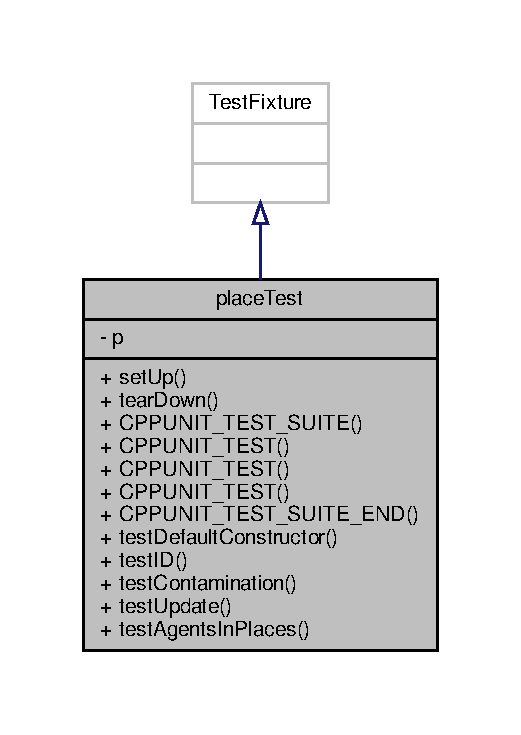
\includegraphics[width=250pt]{classplaceTest__inherit__graph}
\end{center}
\end{figure}


Collaboration diagram for place\+Test\+:\nopagebreak
\begin{figure}[H]
\begin{center}
\leavevmode
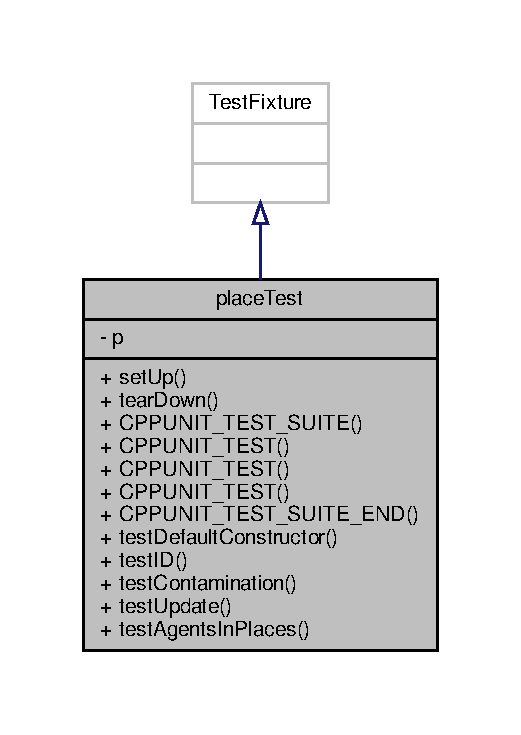
\includegraphics[width=250pt]{classplaceTest__coll__graph}
\end{center}
\end{figure}
\subsection*{Public Member Functions}
\begin{DoxyCompactItemize}
\item 
\mbox{\Hypertarget{classplaceTest_a1818bbe31325c6d9344b35f3b510cacf}\label{classplaceTest_a1818bbe31325c6d9344b35f3b510cacf}} 
void \mbox{\hyperlink{classplaceTest_a1818bbe31325c6d9344b35f3b510cacf}{set\+Up}} ()
\begin{DoxyCompactList}\small\item\em set up a default place pointer \end{DoxyCompactList}\item 
\mbox{\Hypertarget{classplaceTest_a2a0d52566e44cc385dc8fecdae504d6f}\label{classplaceTest_a2a0d52566e44cc385dc8fecdae504d6f}} 
void \mbox{\hyperlink{classplaceTest_a2a0d52566e44cc385dc8fecdae504d6f}{tear\+Down}} ()
\begin{DoxyCompactList}\small\item\em delete the place \end{DoxyCompactList}\item 
\mbox{\Hypertarget{classplaceTest_a48f337cc28990999494a191bd93a0546}\label{classplaceTest_a48f337cc28990999494a191bd93a0546}} 
\mbox{\hyperlink{classplaceTest_a48f337cc28990999494a191bd93a0546}{C\+P\+P\+U\+N\+I\+T\+\_\+\+T\+E\+S\+T\+\_\+\+S\+U\+I\+TE}} (\mbox{\hyperlink{classplaceTest}{place\+Test}})
\begin{DoxyCompactList}\small\item\em automatically create a test suite to add tests to -\/ note this has to come after any setup/tear\+Down \end{DoxyCompactList}\item 
\mbox{\Hypertarget{classplaceTest_ae53796f1cb068709a350189329eb4c95}\label{classplaceTest_ae53796f1cb068709a350189329eb4c95}} 
\mbox{\hyperlink{classplaceTest_ae53796f1cb068709a350189329eb4c95}{C\+P\+P\+U\+N\+I\+T\+\_\+\+T\+E\+ST}} (\mbox{\hyperlink{classplaceTest_a7f6879744d411bded42d786645595245}{test\+Default\+Constructor}})
\begin{DoxyCompactList}\small\item\em check constructor works \end{DoxyCompactList}\item 
\mbox{\Hypertarget{classplaceTest_a1bde1ec54daa7825ca16e8f72473f79a}\label{classplaceTest_a1bde1ec54daa7825ca16e8f72473f79a}} 
\mbox{\hyperlink{classplaceTest_a1bde1ec54daa7825ca16e8f72473f79a}{C\+P\+P\+U\+N\+I\+T\+\_\+\+T\+E\+ST}} (\mbox{\hyperlink{classplaceTest_a1e4e638d2e34b0c247fe82455985aa34}{test\+ID}})
\begin{DoxyCompactList}\small\item\em check place ID \end{DoxyCompactList}\item 
\mbox{\Hypertarget{classplaceTest_a102cedb00ff7312ce527285210eebeff}\label{classplaceTest_a102cedb00ff7312ce527285210eebeff}} 
\mbox{\hyperlink{classplaceTest_a102cedb00ff7312ce527285210eebeff}{C\+P\+P\+U\+N\+I\+T\+\_\+\+T\+E\+ST}} (\mbox{\hyperlink{classplaceTest_a12e071effa88774bb49e498632d19846}{test\+Contamination}})
\begin{DoxyCompactList}\small\item\em test contamination -\/should decay \end{DoxyCompactList}\item 
\mbox{\Hypertarget{classplaceTest_a5f2d3f4fecd70536be029afc85858908}\label{classplaceTest_a5f2d3f4fecd70536be029afc85858908}} 
\mbox{\hyperlink{classplaceTest_a5f2d3f4fecd70536be029afc85858908}{C\+P\+P\+U\+N\+I\+T\+\_\+\+T\+E\+S\+T\+\_\+\+S\+U\+I\+T\+E\+\_\+\+E\+ND}} ()
\begin{DoxyCompactList}\small\item\em test occupancy -\/ currently not used \end{DoxyCompactList}\item 
void \mbox{\hyperlink{classplaceTest_a7f6879744d411bded42d786645595245}{test\+Default\+Constructor}} ()
\begin{DoxyCompactList}\small\item\em The constructor should set the necessary default values. \end{DoxyCompactList}\item 
\mbox{\Hypertarget{classplaceTest_a1e4e638d2e34b0c247fe82455985aa34}\label{classplaceTest_a1e4e638d2e34b0c247fe82455985aa34}} 
void \mbox{\hyperlink{classplaceTest_a1e4e638d2e34b0c247fe82455985aa34}{test\+ID}} ()
\begin{DoxyCompactList}\small\item\em Check the default ID is zero and that it can be set with set\+ID. \end{DoxyCompactList}\item 
void \mbox{\hyperlink{classplaceTest_a12e071effa88774bb49e498632d19846}{test\+Contamination}} ()
\begin{DoxyCompactList}\small\item\em Check the contamination levels. \end{DoxyCompactList}\item 
void \mbox{\hyperlink{classplaceTest_acc20c36b8c0e62cea5068b3707e98237}{test\+Update}} ()
\begin{DoxyCompactList}\small\item\em Check the update exponentially decreases contamination. \end{DoxyCompactList}\item 
void \mbox{\hyperlink{classplaceTest_a095889ea563a243152e41a0e05fffbc2}{test\+Agents\+In\+Places}} ()
\begin{DoxyCompactList}\small\item\em check occupancy \end{DoxyCompactList}\end{DoxyCompactItemize}
\subsection*{Private Attributes}
\begin{DoxyCompactItemize}
\item 
\mbox{\Hypertarget{classplaceTest_a0f4e660bdadc034488490bbadc33e09f}\label{classplaceTest_a0f4e660bdadc034488490bbadc33e09f}} 
place $\ast$ \mbox{\hyperlink{classplaceTest_a0f4e660bdadc034488490bbadc33e09f}{p}}
\begin{DoxyCompactList}\small\item\em A pointer to a default place for the set\+Up method. \end{DoxyCompactList}\end{DoxyCompactItemize}


\subsection{Detailed Description}
Check places for contamination levels and agent occupancy. 

Setting and increase/decrease of contmination is checked, ~\newline
Along with the ability to add and remove agents from the list of occupants 

\subsection{Member Function Documentation}
\mbox{\Hypertarget{classplaceTest_a095889ea563a243152e41a0e05fffbc2}\label{classplaceTest_a095889ea563a243152e41a0e05fffbc2}} 
\index{place\+Test@{place\+Test}!test\+Agents\+In\+Places@{test\+Agents\+In\+Places}}
\index{test\+Agents\+In\+Places@{test\+Agents\+In\+Places}!place\+Test@{place\+Test}}
\subsubsection{\texorpdfstring{test\+Agents\+In\+Places()}{testAgentsInPlaces()}}
{\footnotesize\ttfamily void place\+Test\+::test\+Agents\+In\+Places (\begin{DoxyParamCaption}{ }\end{DoxyParamCaption})\hspace{0.3cm}{\ttfamily [inline]}}



check occupancy 

it should only be possible to add an agent once. removal should not crash if non-\/resident agent is removed.~\newline
number of agents should increase and decrease correctly. The show function shoudl correctly list I\+Ds of residents. \mbox{\Hypertarget{classplaceTest_a12e071effa88774bb49e498632d19846}\label{classplaceTest_a12e071effa88774bb49e498632d19846}} 
\index{place\+Test@{place\+Test}!test\+Contamination@{test\+Contamination}}
\index{test\+Contamination@{test\+Contamination}!place\+Test@{place\+Test}}
\subsubsection{\texorpdfstring{test\+Contamination()}{testContamination()}}
{\footnotesize\ttfamily void place\+Test\+::test\+Contamination (\begin{DoxyParamCaption}{ }\end{DoxyParamCaption})\hspace{0.3cm}{\ttfamily [inline]}}



Check the contamination levels. 

values should increase as expected, not be able to go below zero and get reset to zero by clean\+Contamination() \mbox{\Hypertarget{classplaceTest_a7f6879744d411bded42d786645595245}\label{classplaceTest_a7f6879744d411bded42d786645595245}} 
\index{place\+Test@{place\+Test}!test\+Default\+Constructor@{test\+Default\+Constructor}}
\index{test\+Default\+Constructor@{test\+Default\+Constructor}!place\+Test@{place\+Test}}
\subsubsection{\texorpdfstring{test\+Default\+Constructor()}{testDefaultConstructor()}}
{\footnotesize\ttfamily void place\+Test\+::test\+Default\+Constructor (\begin{DoxyParamCaption}{ }\end{DoxyParamCaption})\hspace{0.3cm}{\ttfamily [inline]}}



The constructor should set the necessary default values. 

use std\+::numeric\+\_\+limits$<$double$>$\+::min() here to find the smallest possible double~\newline
so that test will not fail as a result of rounding errors. \mbox{\Hypertarget{classplaceTest_acc20c36b8c0e62cea5068b3707e98237}\label{classplaceTest_acc20c36b8c0e62cea5068b3707e98237}} 
\index{place\+Test@{place\+Test}!test\+Update@{test\+Update}}
\index{test\+Update@{test\+Update}!place\+Test@{place\+Test}}
\subsubsection{\texorpdfstring{test\+Update()}{testUpdate()}}
{\footnotesize\ttfamily void place\+Test\+::test\+Update (\begin{DoxyParamCaption}{ }\end{DoxyParamCaption})\hspace{0.3cm}{\ttfamily [inline]}}



Check the update exponentially decreases contamination. 

It shoudl aslo be possible to set na diunset the clean\+Contamination flag that makes contamination go to zero after every step (or not, whne it is unset). 

The documentation for this class was generated from the following file\+:\begin{DoxyCompactItemize}
\item 
\mbox{\hyperlink{placetest_8h}{placetest.\+h}}\end{DoxyCompactItemize}

\hypertarget{classrandomTest}{}\section{random\+Test Class Reference}
\label{classrandomTest}\index{random\+Test@{random\+Test}}


Test some of the random number generator behaviour.  




{\ttfamily \#include $<$randomtest.\+h$>$}



Inheritance diagram for random\+Test\+:\nopagebreak
\begin{figure}[H]
\begin{center}
\leavevmode
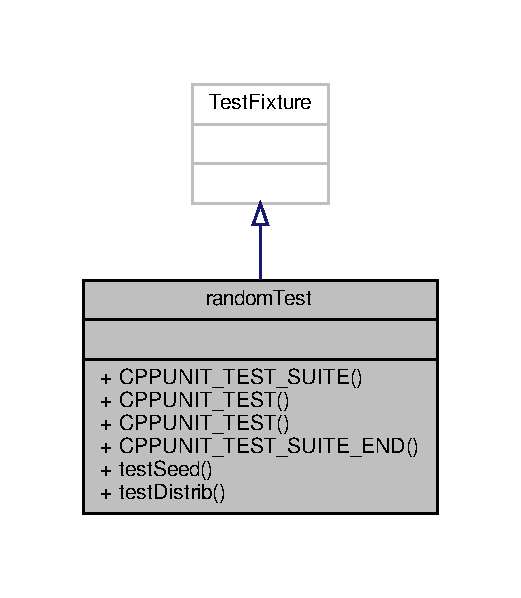
\includegraphics[width=250pt]{classrandomTest__inherit__graph}
\end{center}
\end{figure}


Collaboration diagram for random\+Test\+:\nopagebreak
\begin{figure}[H]
\begin{center}
\leavevmode
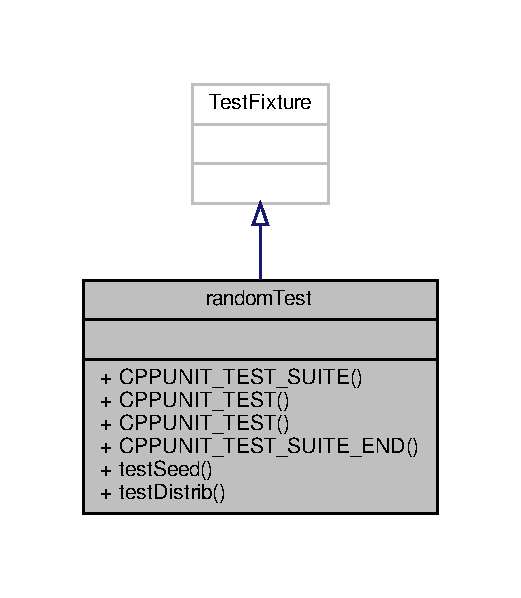
\includegraphics[width=250pt]{classrandomTest__coll__graph}
\end{center}
\end{figure}
\subsection*{Public Member Functions}
\begin{DoxyCompactItemize}
\item 
\mbox{\Hypertarget{classrandomTest_a7cdffcbd64c67232a5cf9a0bc55e3efc}\label{classrandomTest_a7cdffcbd64c67232a5cf9a0bc55e3efc}} 
\mbox{\hyperlink{classrandomTest_a7cdffcbd64c67232a5cf9a0bc55e3efc}{C\+P\+P\+U\+N\+I\+T\+\_\+\+T\+E\+S\+T\+\_\+\+S\+U\+I\+TE}} (\mbox{\hyperlink{classrandomTest}{random\+Test}})
\begin{DoxyCompactList}\small\item\em automatically create a test suite \end{DoxyCompactList}\item 
\mbox{\Hypertarget{classrandomTest_a865784149f2538aba2526748deb2efc8}\label{classrandomTest_a865784149f2538aba2526748deb2efc8}} 
\mbox{\hyperlink{classrandomTest_a865784149f2538aba2526748deb2efc8}{C\+P\+P\+U\+N\+I\+T\+\_\+\+T\+E\+ST}} (\mbox{\hyperlink{classrandomTest_ae7119042c8ecfe9f350cd5b0d6c11906}{test\+Seed}})
\begin{DoxyCompactList}\small\item\em seed test \end{DoxyCompactList}\item 
\mbox{\Hypertarget{classrandomTest_a23f99af2cf532cc659e5b3400dfb052f}\label{classrandomTest_a23f99af2cf532cc659e5b3400dfb052f}} 
\mbox{\hyperlink{classrandomTest_a23f99af2cf532cc659e5b3400dfb052f}{C\+P\+P\+U\+N\+I\+T\+\_\+\+T\+E\+ST}} (\mbox{\hyperlink{classrandomTest_ac6d278a9b086e084f8657453b5e63c07}{test\+Distrib}})
\begin{DoxyCompactList}\small\item\em distribution test \end{DoxyCompactList}\item 
\mbox{\Hypertarget{classrandomTest_a4806098563774b0443bf3e9e994ed904}\label{classrandomTest_a4806098563774b0443bf3e9e994ed904}} 
\mbox{\hyperlink{classrandomTest_a4806098563774b0443bf3e9e994ed904}{C\+P\+P\+U\+N\+I\+T\+\_\+\+T\+E\+S\+T\+\_\+\+S\+U\+I\+T\+E\+\_\+\+E\+ND}} ()
\begin{DoxyCompactList}\small\item\em end test suite \end{DoxyCompactList}\item 
void \mbox{\hyperlink{classrandomTest_ae7119042c8ecfe9f350cd5b0d6c11906}{test\+Seed}} ()
\begin{DoxyCompactList}\small\item\em test random seed behaviour \end{DoxyCompactList}\item 
void \mbox{\hyperlink{classrandomTest_ac6d278a9b086e084f8657453b5e63c07}{test\+Distrib}} ()
\begin{DoxyCompactList}\small\item\em Run through a large number of randoms to see if teh sequence seems uniform-\/ish~\newline
. \end{DoxyCompactList}\end{DoxyCompactItemize}


\subsection{Detailed Description}
Test some of the random number generator behaviour. 

Check the random seed setting works, and try to see whether the distribution of random numbers seems sensible. 

\subsection{Member Function Documentation}
\mbox{\Hypertarget{classrandomTest_ac6d278a9b086e084f8657453b5e63c07}\label{classrandomTest_ac6d278a9b086e084f8657453b5e63c07}} 
\index{random\+Test@{random\+Test}!test\+Distrib@{test\+Distrib}}
\index{test\+Distrib@{test\+Distrib}!random\+Test@{random\+Test}}
\subsubsection{\texorpdfstring{test\+Distrib()}{testDistrib()}}
{\footnotesize\ttfamily void random\+Test\+::test\+Distrib (\begin{DoxyParamCaption}{ }\end{DoxyParamCaption})\hspace{0.3cm}{\ttfamily [inline]}}



Run through a large number of randoms to see if teh sequence seems uniform-\/ish~\newline
. 

The sequence should lie strictly in (0,1). The mean should converge on 0.\+5~\newline
For large number, one might expect the variance about the mean to decrease steadily as the number~\newline
of invocations increases, but instead it steadies at about 0.\+083 -\/ a little consideration reveals~\newline
that the expected variance should indeed converge on 1/12 for a square distribtuion of width 1. \mbox{\Hypertarget{classrandomTest_ae7119042c8ecfe9f350cd5b0d6c11906}\label{classrandomTest_ae7119042c8ecfe9f350cd5b0d6c11906}} 
\index{random\+Test@{random\+Test}!test\+Seed@{test\+Seed}}
\index{test\+Seed@{test\+Seed}!random\+Test@{random\+Test}}
\subsubsection{\texorpdfstring{test\+Seed()}{testSeed()}}
{\footnotesize\ttfamily void random\+Test\+::test\+Seed (\begin{DoxyParamCaption}{ }\end{DoxyParamCaption})\hspace{0.3cm}{\ttfamily [inline]}}



test random seed behaviour 

It is expected that the same random sequence is generated by the same seed. When the seed is reset~\newline
using the set\+Seed method, the random sequence should restart. Each call to the number() method should advance~\newline
the sequence by one step. The constructor should default to seed 0, but allow a seed to be set as an argument. 

The documentation for this class was generated from the following file\+:\begin{DoxyCompactItemize}
\item 
\mbox{\hyperlink{randomtest_8h}{randomtest.\+h}}\end{DoxyCompactItemize}

\hypertarget{classscheduleListTest}{}\section{schedule\+List\+Test Class Reference}
\label{classscheduleListTest}\index{schedule\+List\+Test@{schedule\+List\+Test}}


test out the newclass class  




{\ttfamily \#include $<$schedulelisttest.\+h$>$}



Inheritance diagram for schedule\+List\+Test\+:\nopagebreak
\begin{figure}[H]
\begin{center}
\leavevmode
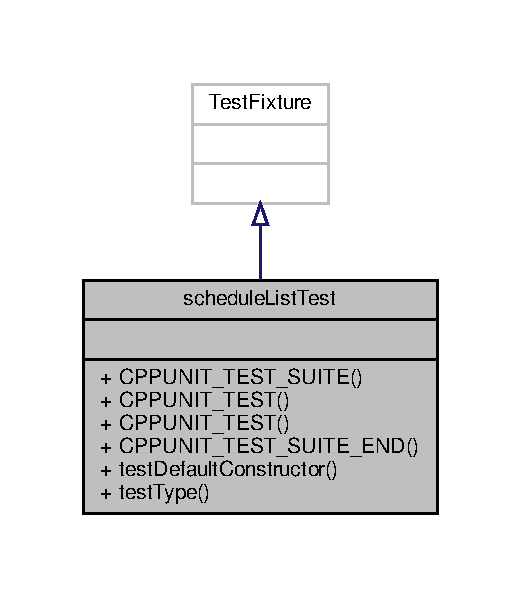
\includegraphics[width=250pt]{classscheduleListTest__inherit__graph}
\end{center}
\end{figure}


Collaboration diagram for schedule\+List\+Test\+:\nopagebreak
\begin{figure}[H]
\begin{center}
\leavevmode
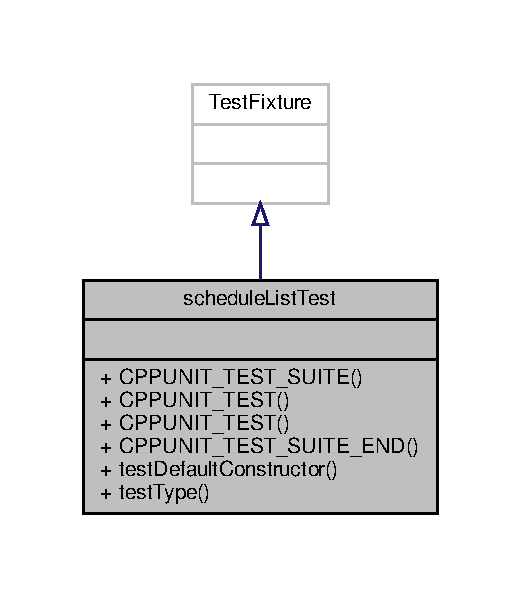
\includegraphics[width=250pt]{classscheduleListTest__coll__graph}
\end{center}
\end{figure}
\subsection*{Public Member Functions}
\begin{DoxyCompactItemize}
\item 
\mbox{\Hypertarget{classscheduleListTest_a072cf6a160cc6694ac384345165c4f0b}\label{classscheduleListTest_a072cf6a160cc6694ac384345165c4f0b}} 
\mbox{\hyperlink{classscheduleListTest_a072cf6a160cc6694ac384345165c4f0b}{C\+P\+P\+U\+N\+I\+T\+\_\+\+T\+E\+S\+T\+\_\+\+S\+U\+I\+TE}} (\mbox{\hyperlink{classscheduleListTest}{schedule\+List\+Test}})
\begin{DoxyCompactList}\small\item\em automatically create a test suite to add tests to \end{DoxyCompactList}\item 
\mbox{\Hypertarget{classscheduleListTest_abaa94007bd8e605dc3741c3c216f9c27}\label{classscheduleListTest_abaa94007bd8e605dc3741c3c216f9c27}} 
\mbox{\hyperlink{classscheduleListTest_abaa94007bd8e605dc3741c3c216f9c27}{C\+P\+P\+U\+N\+I\+T\+\_\+\+T\+E\+ST}} (\mbox{\hyperlink{classscheduleListTest_a8495411fca3065150fb4ab98b4d950eb}{test\+Default\+Constructor}})
\begin{DoxyCompactList}\small\item\em test the default constructor \end{DoxyCompactList}\item 
\mbox{\Hypertarget{classscheduleListTest_a6291991f154c56d50fee42dfb5809d7d}\label{classscheduleListTest_a6291991f154c56d50fee42dfb5809d7d}} 
\mbox{\hyperlink{classscheduleListTest_a6291991f154c56d50fee42dfb5809d7d}{C\+P\+P\+U\+N\+I\+T\+\_\+\+T\+E\+ST}} (\mbox{\hyperlink{classscheduleListTest_a420ec9f4f0d97230ebe2911d5be4a856}{test\+Type}})
\begin{DoxyCompactList}\small\item\em check correct types are returned from string arguments \end{DoxyCompactList}\item 
\mbox{\Hypertarget{classscheduleListTest_a161be3834e2145e52cae28a5cb79d45c}\label{classscheduleListTest_a161be3834e2145e52cae28a5cb79d45c}} 
\mbox{\hyperlink{classscheduleListTest_a161be3834e2145e52cae28a5cb79d45c}{C\+P\+P\+U\+N\+I\+T\+\_\+\+T\+E\+S\+T\+\_\+\+S\+U\+I\+T\+E\+\_\+\+E\+ND}} ()
\begin{DoxyCompactList}\small\item\em end the test suite \end{DoxyCompactList}\item 
void \mbox{\hyperlink{classscheduleListTest_a8495411fca3065150fb4ab98b4d950eb}{test\+Default\+Constructor}} ()
\begin{DoxyCompactList}\small\item\em make sure results from constructor are as expected \end{DoxyCompactList}\item 
void \mbox{\hyperlink{classscheduleListTest_a420ec9f4f0d97230ebe2911d5be4a856}{test\+Type}} ()
\begin{DoxyCompactList}\small\item\em check that string names of schedules convert correctly to the schedule\+List types \end{DoxyCompactList}\end{DoxyCompactItemize}


\subsection{Detailed Description}
test out the newclass class 

what this does 

\subsection{Member Function Documentation}
\mbox{\Hypertarget{classscheduleListTest_a8495411fca3065150fb4ab98b4d950eb}\label{classscheduleListTest_a8495411fca3065150fb4ab98b4d950eb}} 
\index{schedule\+List\+Test@{schedule\+List\+Test}!test\+Default\+Constructor@{test\+Default\+Constructor}}
\index{test\+Default\+Constructor@{test\+Default\+Constructor}!schedule\+List\+Test@{schedule\+List\+Test}}
\subsubsection{\texorpdfstring{test\+Default\+Constructor()}{testDefaultConstructor()}}
{\footnotesize\ttfamily void schedule\+List\+Test\+::test\+Default\+Constructor (\begin{DoxyParamCaption}{ }\end{DoxyParamCaption})\hspace{0.3cm}{\ttfamily [inline]}}



make sure results from constructor are as expected 

there should be one mobile and one stationary schedule \mbox{\Hypertarget{classscheduleListTest_a420ec9f4f0d97230ebe2911d5be4a856}\label{classscheduleListTest_a420ec9f4f0d97230ebe2911d5be4a856}} 
\index{schedule\+List\+Test@{schedule\+List\+Test}!test\+Type@{test\+Type}}
\index{test\+Type@{test\+Type}!schedule\+List\+Test@{schedule\+List\+Test}}
\subsubsection{\texorpdfstring{test\+Type()}{testType()}}
{\footnotesize\ttfamily void schedule\+List\+Test\+::test\+Type (\begin{DoxyParamCaption}{ }\end{DoxyParamCaption})\hspace{0.3cm}{\ttfamily [inline]}}



check that string names of schedules convert correctly to the schedule\+List types 

check \char`\"{}mobile\char`\"{} and \char`\"{}stationary\char`\"{} incorrect names shoudl default to stationary 

The documentation for this class was generated from the following file\+:\begin{DoxyCompactItemize}
\item 
\mbox{\hyperlink{schedulelisttest_8h}{schedulelisttest.\+h}}\end{DoxyCompactItemize}

\hypertarget{classtimeReporterTest}{}\section{time\+Reporter\+Test Class Reference}
\label{classtimeReporterTest}\index{time\+Reporter\+Test@{time\+Reporter\+Test}}


Check intervals are computed and reported as expected.  




{\ttfamily \#include $<$timereportertest.\+h$>$}



Inheritance diagram for time\+Reporter\+Test\+:\nopagebreak
\begin{figure}[H]
\begin{center}
\leavevmode
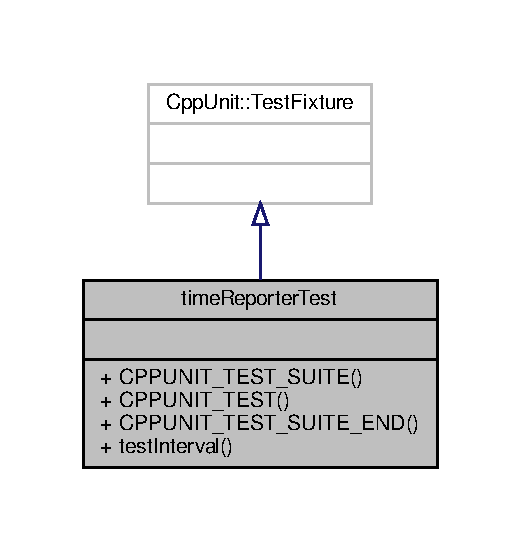
\includegraphics[width=250pt]{classtimeReporterTest__inherit__graph}
\end{center}
\end{figure}


Collaboration diagram for time\+Reporter\+Test\+:\nopagebreak
\begin{figure}[H]
\begin{center}
\leavevmode
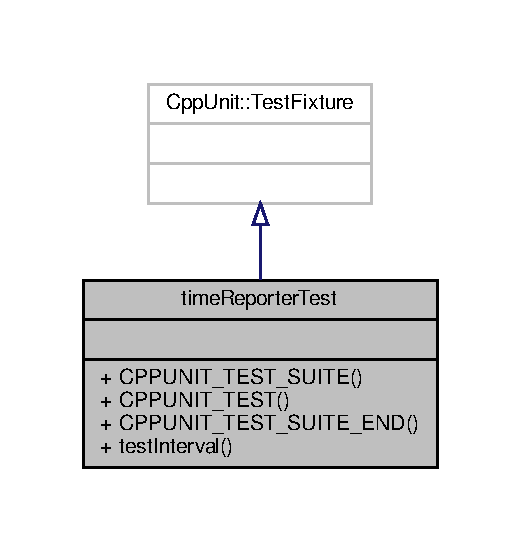
\includegraphics[width=250pt]{classtimeReporterTest__coll__graph}
\end{center}
\end{figure}
\subsection*{Public Member Functions}
\begin{DoxyCompactItemize}
\item 
\mbox{\Hypertarget{classtimeReporterTest_a21439462ca34e21b52c2f535cd30e192}\label{classtimeReporterTest_a21439462ca34e21b52c2f535cd30e192}} 
\mbox{\hyperlink{classtimeReporterTest_a21439462ca34e21b52c2f535cd30e192}{C\+P\+P\+U\+N\+I\+T\+\_\+\+T\+E\+S\+T\+\_\+\+S\+U\+I\+TE}} (\mbox{\hyperlink{classtimeReporterTest}{time\+Reporter\+Test}})
\begin{DoxyCompactList}\small\item\em automatically create a test suite \end{DoxyCompactList}\item 
\mbox{\Hypertarget{classtimeReporterTest_a73cb289025e42913a59225e5b1530119}\label{classtimeReporterTest_a73cb289025e42913a59225e5b1530119}} 
\mbox{\hyperlink{classtimeReporterTest_a73cb289025e42913a59225e5b1530119}{C\+P\+P\+U\+N\+I\+T\+\_\+\+T\+E\+ST}} (\mbox{\hyperlink{classtimeReporterTest_a4488d70ca37d086b82cce74e5c25a53d}{test\+Interval}})
\begin{DoxyCompactList}\small\item\em check that intervals are measured correctly \end{DoxyCompactList}\item 
\mbox{\Hypertarget{classtimeReporterTest_a603425c4735cb3300643da88aa75ed3b}\label{classtimeReporterTest_a603425c4735cb3300643da88aa75ed3b}} 
\mbox{\hyperlink{classtimeReporterTest_a603425c4735cb3300643da88aa75ed3b}{C\+P\+P\+U\+N\+I\+T\+\_\+\+T\+E\+S\+T\+\_\+\+S\+U\+I\+T\+E\+\_\+\+E\+ND}} ()
\begin{DoxyCompactList}\small\item\em end test suite \end{DoxyCompactList}\item 
void \mbox{\hyperlink{classtimeReporterTest_a4488d70ca37d086b82cce74e5c25a53d}{test\+Interval}} ()
\begin{DoxyCompactList}\small\item\em Check that wating for a few milliseconds is correctly reported. \end{DoxyCompactList}\end{DoxyCompactItemize}


\subsection{Detailed Description}
Check intervals are computed and reported as expected. 

\subsection{Member Function Documentation}
\mbox{\Hypertarget{classtimeReporterTest_a4488d70ca37d086b82cce74e5c25a53d}\label{classtimeReporterTest_a4488d70ca37d086b82cce74e5c25a53d}} 
\index{time\+Reporter\+Test@{time\+Reporter\+Test}!test\+Interval@{test\+Interval}}
\index{test\+Interval@{test\+Interval}!time\+Reporter\+Test@{time\+Reporter\+Test}}
\subsubsection{\texorpdfstring{test\+Interval()}{testInterval()}}
{\footnotesize\ttfamily void time\+Reporter\+Test\+::test\+Interval (\begin{DoxyParamCaption}{ }\end{DoxyParamCaption})\hspace{0.3cm}{\ttfamily [inline]}}



Check that wating for a few milliseconds is correctly reported. 

uses the usleep function to wait a specified number of microseconds between two calls to time\+Reporter\+::get\+Time ~\newline
Tests the timereporter interval function to be sure it is always positive.\+Then outputs some text for the user to check ~\newline
that the reporting is as expected (since show\+Interval should write to stdout) 

The documentation for this class was generated from the following file\+:\begin{DoxyCompactItemize}
\item 
\mbox{\hyperlink{timereportertest_8h}{timereportertest.\+h}}\end{DoxyCompactItemize}

\hypertarget{classtimeStepTest}{}\section{time\+Step\+Test Class Reference}
\label{classtimeStepTest}\index{time\+Step\+Test@{time\+Step\+Test}}


Check the class that maps the time step to a given set of real-\/world units (e.\+g. hours)  




{\ttfamily \#include $<$timesteptest.\+h$>$}



Inheritance diagram for time\+Step\+Test\+:
\nopagebreak
\begin{figure}[H]
\begin{center}
\leavevmode
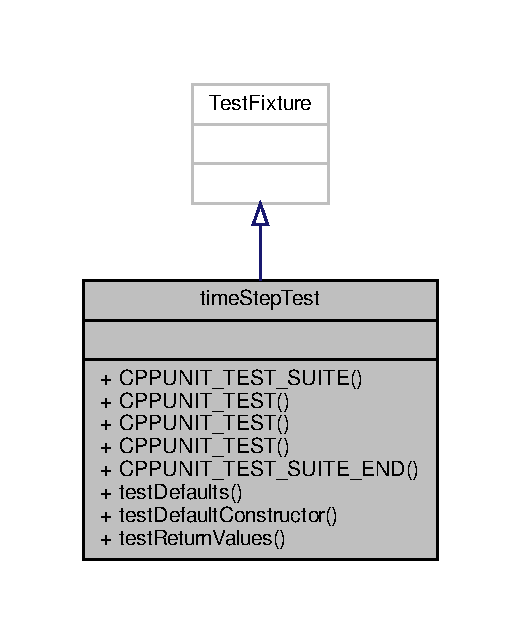
\includegraphics[width=250pt]{classtimeStepTest__inherit__graph}
\end{center}
\end{figure}


Collaboration diagram for time\+Step\+Test\+:
\nopagebreak
\begin{figure}[H]
\begin{center}
\leavevmode
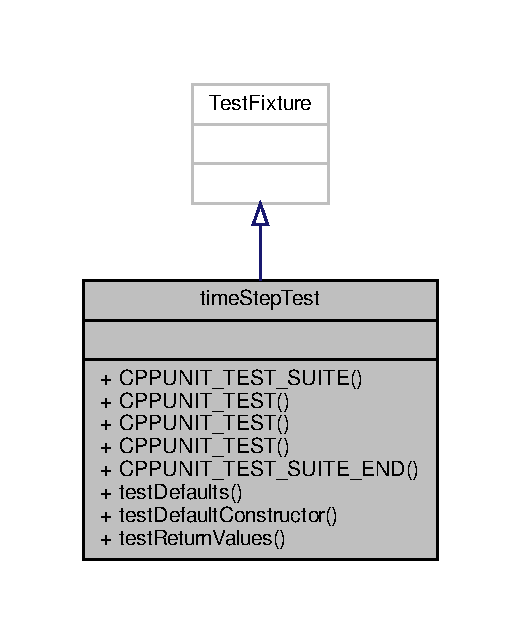
\includegraphics[width=250pt]{classtimeStepTest__coll__graph}
\end{center}
\end{figure}
\subsection*{Public Member Functions}
\begin{DoxyCompactItemize}
\item 
\mbox{\Hypertarget{classtimeStepTest_a33172d5eb5f67ad6eb8ef3e04baed49c}\label{classtimeStepTest_a33172d5eb5f67ad6eb8ef3e04baed49c}} 
\mbox{\hyperlink{classtimeStepTest_a33172d5eb5f67ad6eb8ef3e04baed49c}{C\+P\+P\+U\+N\+I\+T\+\_\+\+T\+E\+S\+T\+\_\+\+S\+U\+I\+TE}} (\mbox{\hyperlink{classtimeStepTest}{time\+Step\+Test}})
\begin{DoxyCompactList}\small\item\em automatically create a test suite to add tests to -\/ note this has to come after any setup/tear\+Down \end{DoxyCompactList}\item 
\mbox{\Hypertarget{classtimeStepTest_af38279a078dff48ea04654c02d8b5486}\label{classtimeStepTest_af38279a078dff48ea04654c02d8b5486}} 
\mbox{\hyperlink{classtimeStepTest_af38279a078dff48ea04654c02d8b5486}{C\+P\+P\+U\+N\+I\+T\+\_\+\+T\+E\+ST}} (\mbox{\hyperlink{classtimeStepTest_a8853eb9214716d678e9c341470582fec}{test\+Stepping}})
\begin{DoxyCompactList}\small\item\em check time step number updates correctly \end{DoxyCompactList}\item 
\mbox{\Hypertarget{classtimeStepTest_a8dd61267ca389d04a8db4776b64eee9a}\label{classtimeStepTest_a8dd61267ca389d04a8db4776b64eee9a}} 
\mbox{\hyperlink{classtimeStepTest_a8dd61267ca389d04a8db4776b64eee9a}{C\+P\+P\+U\+N\+I\+T\+\_\+\+T\+E\+ST}} (\mbox{\hyperlink{classtimeStepTest_ae501f2f63633a2b24c4cfc1f9c33f96b}{test\+Defaults}})
\begin{DoxyCompactList}\small\item\em test the default state \end{DoxyCompactList}\item 
\mbox{\Hypertarget{classtimeStepTest_a215e48294ca13fb21cd703e31e80bf48}\label{classtimeStepTest_a215e48294ca13fb21cd703e31e80bf48}} 
\mbox{\hyperlink{classtimeStepTest_a215e48294ca13fb21cd703e31e80bf48}{C\+P\+P\+U\+N\+I\+T\+\_\+\+T\+E\+ST}} (\mbox{\hyperlink{classtimeStepTest_a3e6e3abcb3b887cd3ebbbacb3c6a812f}{test\+Default\+Constructor}})
\begin{DoxyCompactList}\small\item\em check the constructor works used on an object \end{DoxyCompactList}\item 
\mbox{\Hypertarget{classtimeStepTest_a83693f088afb5b02ca85ede22866efbf}\label{classtimeStepTest_a83693f088afb5b02ca85ede22866efbf}} 
\mbox{\hyperlink{classtimeStepTest_a83693f088afb5b02ca85ede22866efbf}{C\+P\+P\+U\+N\+I\+T\+\_\+\+T\+E\+ST}} (\mbox{\hyperlink{classtimeStepTest_abb17f1970e1ec459c524ef87870f651f}{test\+Return\+Values}})
\begin{DoxyCompactList}\small\item\em check that all the functions related to the timestep work \end{DoxyCompactList}\item 
\mbox{\Hypertarget{classtimeStepTest_aac5a656f3c6d28ffce6db8d6e05e3f7d}\label{classtimeStepTest_aac5a656f3c6d28ffce6db8d6e05e3f7d}} 
\mbox{\hyperlink{classtimeStepTest_aac5a656f3c6d28ffce6db8d6e05e3f7d}{C\+P\+P\+U\+N\+I\+T\+\_\+\+T\+E\+ST}} (\mbox{\hyperlink{classtimeStepTest_a35fe812055dc5fa7f53eb898d568256c}{test\+Date\+Functions}})
\begin{DoxyCompactList}\small\item\em check that all date functionality works \end{DoxyCompactList}\item 
\mbox{\Hypertarget{classtimeStepTest_a9d77630b4ebb30faacc9627d0739c836}\label{classtimeStepTest_a9d77630b4ebb30faacc9627d0739c836}} 
\mbox{\hyperlink{classtimeStepTest_a9d77630b4ebb30faacc9627d0739c836}{C\+P\+P\+U\+N\+I\+T\+\_\+\+T\+E\+S\+T\+\_\+\+S\+U\+I\+T\+E\+\_\+\+E\+ND}} ()
\begin{DoxyCompactList}\small\item\em end test suite \end{DoxyCompactList}\item 
void \mbox{\hyperlink{classtimeStepTest_a8853eb9214716d678e9c341470582fec}{test\+Stepping}} ()
\begin{DoxyCompactList}\small\item\em Check that the time step number updates as expected. \end{DoxyCompactList}\item 
\mbox{\Hypertarget{classtimeStepTest_ae501f2f63633a2b24c4cfc1f9c33f96b}\label{classtimeStepTest_ae501f2f63633a2b24c4cfc1f9c33f96b}} 
void \mbox{\hyperlink{classtimeStepTest_ae501f2f63633a2b24c4cfc1f9c33f96b}{test\+Defaults}} ()
\begin{DoxyCompactList}\small\item\em as a static class the static variable should have values as in time\+Step.\+cpp \end{DoxyCompactList}\item 
\mbox{\Hypertarget{classtimeStepTest_a3e6e3abcb3b887cd3ebbbacb3c6a812f}\label{classtimeStepTest_a3e6e3abcb3b887cd3ebbbacb3c6a812f}} 
void \mbox{\hyperlink{classtimeStepTest_a3e6e3abcb3b887cd3ebbbacb3c6a812f}{test\+Default\+Constructor}} ()
\begin{DoxyCompactList}\small\item\em When an object is created, the values should be those from the constructor in time\+Step.\+h. \end{DoxyCompactList}\item 
void \mbox{\hyperlink{classtimeStepTest_abb17f1970e1ec459c524ef87870f651f}{test\+Return\+Values}} ()
\begin{DoxyCompactList}\small\item\em Check that the return values are as expected. \end{DoxyCompactList}\item 
void \mbox{\hyperlink{classtimeStepTest_a35fe812055dc5fa7f53eb898d568256c}{test\+Date\+Functions}} ()
\begin{DoxyCompactList}\small\item\em Check daet calculations. \end{DoxyCompactList}\end{DoxyCompactItemize}


\subsection{Detailed Description}
Check the class that maps the time step to a given set of real-\/world units (e.\+g. hours) 

NB if time\+Step\+::deltaT is reset anywhere, because timestep is a static class, this can affect other tests 

\subsection{Member Function Documentation}
\mbox{\Hypertarget{classtimeStepTest_a35fe812055dc5fa7f53eb898d568256c}\label{classtimeStepTest_a35fe812055dc5fa7f53eb898d568256c}} 
\index{time\+Step\+Test@{time\+Step\+Test}!test\+Date\+Functions@{test\+Date\+Functions}}
\index{test\+Date\+Functions@{test\+Date\+Functions}!time\+Step\+Test@{time\+Step\+Test}}
\subsubsection{\texorpdfstring{test\+Date\+Functions()}{testDateFunctions()}}
{\footnotesize\ttfamily void time\+Step\+Test\+::test\+Date\+Functions (\begin{DoxyParamCaption}{ }\end{DoxyParamCaption})\hspace{0.3cm}{\ttfamily [inline]}}



Check daet calculations. 

Check the weekday calcualtor works for some known days \mbox{\Hypertarget{classtimeStepTest_abb17f1970e1ec459c524ef87870f651f}\label{classtimeStepTest_abb17f1970e1ec459c524ef87870f651f}} 
\index{time\+Step\+Test@{time\+Step\+Test}!test\+Return\+Values@{test\+Return\+Values}}
\index{test\+Return\+Values@{test\+Return\+Values}!time\+Step\+Test@{time\+Step\+Test}}
\subsubsection{\texorpdfstring{test\+Return\+Values()}{testReturnValues()}}
{\footnotesize\ttfamily void time\+Step\+Test\+::test\+Return\+Values (\begin{DoxyParamCaption}{ }\end{DoxyParamCaption})\hspace{0.3cm}{\ttfamily [inline]}}



Check that the return values are as expected. 

e.\+g. after setting time\+Step\+::setdelta\+T(time\+Step\+::hour()), Time\+Steps\+Per\+Hour and hours\+Per\+Time\+Step should both be 1 \mbox{\Hypertarget{classtimeStepTest_a8853eb9214716d678e9c341470582fec}\label{classtimeStepTest_a8853eb9214716d678e9c341470582fec}} 
\index{time\+Step\+Test@{time\+Step\+Test}!test\+Stepping@{test\+Stepping}}
\index{test\+Stepping@{test\+Stepping}!time\+Step\+Test@{time\+Step\+Test}}
\subsubsection{\texorpdfstring{test\+Stepping()}{testStepping()}}
{\footnotesize\ttfamily void time\+Step\+Test\+::test\+Stepping (\begin{DoxyParamCaption}{ }\end{DoxyParamCaption})\hspace{0.3cm}{\ttfamily [inline]}}



Check that the time step number updates as expected. 

should start at 0 and advance by one on every call to update. Make sure this is the first test so that calls to update haven\textquotesingle{}t happened yet 

The documentation for this class was generated from the following file\+:\begin{DoxyCompactItemize}
\item 
\mbox{\hyperlink{timesteptest_8h}{timesteptest.\+h}}\end{DoxyCompactItemize}

\hypertarget{classtravelScheduleTest}{}\section{travel\+Schedule\+Test Class Reference}
\label{classtravelScheduleTest}\index{travel\+Schedule\+Test@{travel\+Schedule\+Test}}


Exercise the fixed travel schedules.  




{\ttfamily \#include $<$travelscheduletest.\+h$>$}



Inheritance diagram for travel\+Schedule\+Test\+:\nopagebreak
\begin{figure}[H]
\begin{center}
\leavevmode
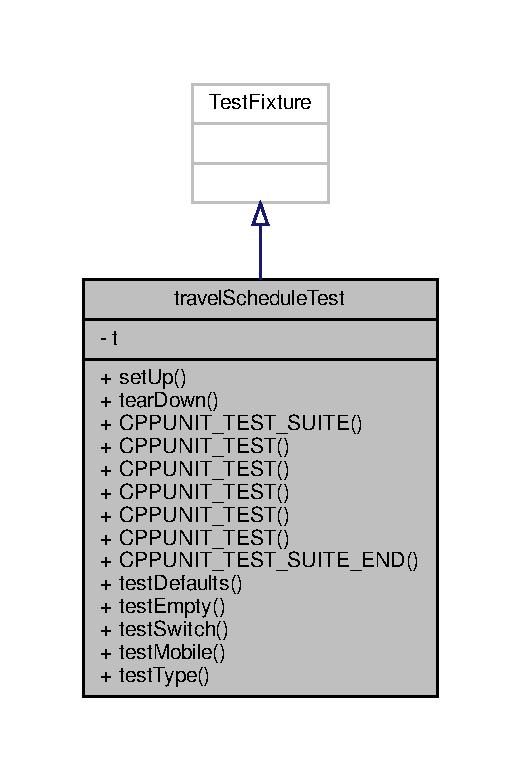
\includegraphics[width=250pt]{classtravelScheduleTest__inherit__graph}
\end{center}
\end{figure}


Collaboration diagram for travel\+Schedule\+Test\+:\nopagebreak
\begin{figure}[H]
\begin{center}
\leavevmode
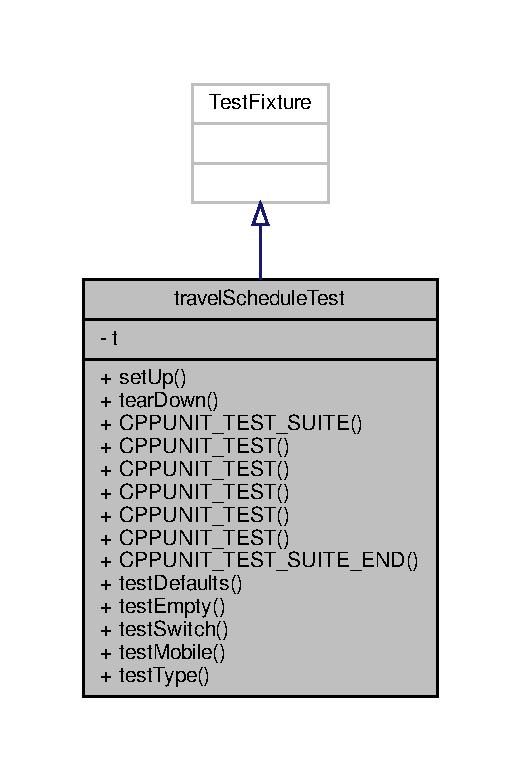
\includegraphics[width=250pt]{classtravelScheduleTest__coll__graph}
\end{center}
\end{figure}
\subsection*{Public Member Functions}
\begin{DoxyCompactItemize}
\item 
\mbox{\Hypertarget{classtravelScheduleTest_ad43113c0f75ff6969e57fb865975d133}\label{classtravelScheduleTest_ad43113c0f75ff6969e57fb865975d133}} 
void \mbox{\hyperlink{classtravelScheduleTest_ad43113c0f75ff6969e57fb865975d133}{set\+Up}} ()
\begin{DoxyCompactList}\small\item\em set up a default travel schedule pointer (stationary at home) \end{DoxyCompactList}\item 
\mbox{\Hypertarget{classtravelScheduleTest_a69320630d353404c79e158289c5d73f4}\label{classtravelScheduleTest_a69320630d353404c79e158289c5d73f4}} 
void \mbox{\hyperlink{classtravelScheduleTest_a69320630d353404c79e158289c5d73f4}{tear\+Down}} ()
\begin{DoxyCompactList}\small\item\em delete the schedule \end{DoxyCompactList}\item 
\mbox{\Hypertarget{classtravelScheduleTest_a019e7ca232e9bdbe438ac24da88dc158}\label{classtravelScheduleTest_a019e7ca232e9bdbe438ac24da88dc158}} 
\mbox{\hyperlink{classtravelScheduleTest_a019e7ca232e9bdbe438ac24da88dc158}{C\+P\+P\+U\+N\+I\+T\+\_\+\+T\+E\+S\+T\+\_\+\+S\+U\+I\+TE}} (\mbox{\hyperlink{classtravelScheduleTest}{travel\+Schedule\+Test}})
\begin{DoxyCompactList}\small\item\em automatically create a test suite to add tests to -\/ note this has to come after any setup/tear\+Down \end{DoxyCompactList}\item 
\mbox{\Hypertarget{classtravelScheduleTest_ab715d40df88ffedf9f304c9aa7b17b71}\label{classtravelScheduleTest_ab715d40df88ffedf9f304c9aa7b17b71}} 
\mbox{\hyperlink{classtravelScheduleTest_ab715d40df88ffedf9f304c9aa7b17b71}{C\+P\+P\+U\+N\+I\+T\+\_\+\+T\+E\+ST}} (\mbox{\hyperlink{classtravelScheduleTest_a20320a46b0a0a9cd70e643f1ebe0ee0a}{test\+Defaults}})
\begin{DoxyCompactList}\small\item\em add test of defaults to the suite \end{DoxyCompactList}\item 
\mbox{\Hypertarget{classtravelScheduleTest_ac324ee93bd9a16956c54af66aad6ebc8}\label{classtravelScheduleTest_ac324ee93bd9a16956c54af66aad6ebc8}} 
\mbox{\hyperlink{classtravelScheduleTest_ac324ee93bd9a16956c54af66aad6ebc8}{C\+P\+P\+U\+N\+I\+T\+\_\+\+T\+E\+ST}} (\mbox{\hyperlink{classtravelScheduleTest_a9a54489b2ffb494a08bbcfa9391e0c8d}{test\+Empty}})
\begin{DoxyCompactList}\small\item\em test of empty schedule \end{DoxyCompactList}\item 
\mbox{\Hypertarget{classtravelScheduleTest_a167d28d507e5146c0fa7adbac5003870}\label{classtravelScheduleTest_a167d28d507e5146c0fa7adbac5003870}} 
\mbox{\hyperlink{classtravelScheduleTest_a167d28d507e5146c0fa7adbac5003870}{C\+P\+P\+U\+N\+I\+T\+\_\+\+T\+E\+ST}} (\mbox{\hyperlink{classtravelScheduleTest_afa04fc9d3f86668e36c74a1f27c2d5aa}{test\+Switch}})
\begin{DoxyCompactList}\small\item\em test schedule switching \end{DoxyCompactList}\item 
\mbox{\Hypertarget{classtravelScheduleTest_a5d6627a9c80540df8f28f265d9852152}\label{classtravelScheduleTest_a5d6627a9c80540df8f28f265d9852152}} 
\mbox{\hyperlink{classtravelScheduleTest_a5d6627a9c80540df8f28f265d9852152}{C\+P\+P\+U\+N\+I\+T\+\_\+\+T\+E\+ST}} (\mbox{\hyperlink{classtravelScheduleTest_a7d457e4ae5c44853c450860284993a57}{test\+Mobile}})
\begin{DoxyCompactList}\small\item\em test mobile schedule \end{DoxyCompactList}\item 
\mbox{\Hypertarget{classtravelScheduleTest_aad272e8dae22e4faffdd408f34a71505}\label{classtravelScheduleTest_aad272e8dae22e4faffdd408f34a71505}} 
\mbox{\hyperlink{classtravelScheduleTest_aad272e8dae22e4faffdd408f34a71505}{C\+P\+P\+U\+N\+I\+T\+\_\+\+T\+E\+ST}} (\mbox{\hyperlink{classtravelScheduleTest_a66b5ac55f22c6d892798936d634d2316}{test\+Type}})
\begin{DoxyCompactList}\small\item\em test alternate constructors using types \end{DoxyCompactList}\item 
\mbox{\Hypertarget{classtravelScheduleTest_a25f18ca31d145e1e4826d7d293de7355}\label{classtravelScheduleTest_a25f18ca31d145e1e4826d7d293de7355}} 
\mbox{\hyperlink{classtravelScheduleTest_a25f18ca31d145e1e4826d7d293de7355}{C\+P\+P\+U\+N\+I\+T\+\_\+\+T\+E\+S\+T\+\_\+\+S\+U\+I\+T\+E\+\_\+\+E\+ND}} ()
\begin{DoxyCompactList}\small\item\em end the test suite \end{DoxyCompactList}\item 
\mbox{\Hypertarget{classtravelScheduleTest_a20320a46b0a0a9cd70e643f1ebe0ee0a}\label{classtravelScheduleTest_a20320a46b0a0a9cd70e643f1ebe0ee0a}} 
void \mbox{\hyperlink{classtravelScheduleTest_a20320a46b0a0a9cd70e643f1ebe0ee0a}{test\+Defaults}} ()
\begin{DoxyCompactList}\small\item\em check the default schedule is as expected -\/ make sure the destinations and timings are correct \end{DoxyCompactList}\item 
\mbox{\Hypertarget{classtravelScheduleTest_a9a54489b2ffb494a08bbcfa9391e0c8d}\label{classtravelScheduleTest_a9a54489b2ffb494a08bbcfa9391e0c8d}} 
void \mbox{\hyperlink{classtravelScheduleTest_a9a54489b2ffb494a08bbcfa9391e0c8d}{test\+Empty}} ()
\begin{DoxyCompactList}\small\item\em make sure the schedule behaves smoothly if empty (the agent stays at home the whole time \end{DoxyCompactList}\item 
void \mbox{\hyperlink{classtravelScheduleTest_afa04fc9d3f86668e36c74a1f27c2d5aa}{test\+Switch}} ()
\begin{DoxyCompactList}\small\item\em check that incorrect schedule names have no effect and check switching works . \end{DoxyCompactList}\item 
void \mbox{\hyperlink{classtravelScheduleTest_a7d457e4ae5c44853c450860284993a57}{test\+Mobile}} ()
\begin{DoxyCompactList}\small\item\em exercise the mobile schedule \end{DoxyCompactList}\item 
void \mbox{\hyperlink{classtravelScheduleTest_a66b5ac55f22c6d892798936d634d2316}{test\+Type}} ()
\begin{DoxyCompactList}\small\item\em check that the mobile and stationary schedules are picked up correctly in the constructor \end{DoxyCompactList}\end{DoxyCompactItemize}
\subsection*{Private Attributes}
\begin{DoxyCompactItemize}
\item 
\mbox{\Hypertarget{classtravelScheduleTest_a98d861ced2b339627f69fd5d5f343743}\label{classtravelScheduleTest_a98d861ced2b339627f69fd5d5f343743}} 
travel\+Schedule $\ast$ \mbox{\hyperlink{classtravelScheduleTest_a98d861ced2b339627f69fd5d5f343743}{t}}
\begin{DoxyCompactList}\small\item\em A pointer to a default schedule for the set\+Up method. \end{DoxyCompactList}\end{DoxyCompactItemize}


\subsection{Detailed Description}
Exercise the fixed travel schedules. 

Check that switching between schedules resets each to the start.~\newline
Check the destinations and timings are as expected. 

\subsection{Member Function Documentation}
\mbox{\Hypertarget{classtravelScheduleTest_a7d457e4ae5c44853c450860284993a57}\label{classtravelScheduleTest_a7d457e4ae5c44853c450860284993a57}} 
\index{travel\+Schedule\+Test@{travel\+Schedule\+Test}!test\+Mobile@{test\+Mobile}}
\index{test\+Mobile@{test\+Mobile}!travel\+Schedule\+Test@{travel\+Schedule\+Test}}
\subsubsection{\texorpdfstring{test\+Mobile()}{testMobile()}}
{\footnotesize\ttfamily void travel\+Schedule\+Test\+::test\+Mobile (\begin{DoxyParamCaption}{ }\end{DoxyParamCaption})\hspace{0.3cm}{\ttfamily [inline]}}



exercise the mobile schedule 

run completely through the schedule making sure it wraps round to the start again after a day ~\newline
\mbox{\Hypertarget{classtravelScheduleTest_afa04fc9d3f86668e36c74a1f27c2d5aa}\label{classtravelScheduleTest_afa04fc9d3f86668e36c74a1f27c2d5aa}} 
\index{travel\+Schedule\+Test@{travel\+Schedule\+Test}!test\+Switch@{test\+Switch}}
\index{test\+Switch@{test\+Switch}!travel\+Schedule\+Test@{travel\+Schedule\+Test}}
\subsubsection{\texorpdfstring{test\+Switch()}{testSwitch()}}
{\footnotesize\ttfamily void travel\+Schedule\+Test\+::test\+Switch (\begin{DoxyParamCaption}{ }\end{DoxyParamCaption})\hspace{0.3cm}{\ttfamily [inline]}}



check that incorrect schedule names have no effect and check switching works . 

Switch to a mobile schedule and run through it a bit, then switch back to stationary ~\newline
\mbox{\Hypertarget{classtravelScheduleTest_a66b5ac55f22c6d892798936d634d2316}\label{classtravelScheduleTest_a66b5ac55f22c6d892798936d634d2316}} 
\index{travel\+Schedule\+Test@{travel\+Schedule\+Test}!test\+Type@{test\+Type}}
\index{test\+Type@{test\+Type}!travel\+Schedule\+Test@{travel\+Schedule\+Test}}
\subsubsection{\texorpdfstring{test\+Type()}{testType()}}
{\footnotesize\ttfamily void travel\+Schedule\+Test\+::test\+Type (\begin{DoxyParamCaption}{ }\end{DoxyParamCaption})\hspace{0.3cm}{\ttfamily [inline]}}



check that the mobile and stationary schedules are picked up correctly in the constructor 

the non-\/default constructor should use the type from schedule list to pick out one of the defined schedules 

The documentation for this class was generated from the following file\+:\begin{DoxyCompactItemize}
\item 
\mbox{\hyperlink{travelscheduletest_8h}{travelscheduletest.\+h}}\end{DoxyCompactItemize}

\chapter{File Documentation}
\hypertarget{agenttest_8h}{}\section{agenttest.\+h File Reference}
\label{agenttest_8h}\index{agenttest.\+h@{agenttest.\+h}}


File containing the definition of the \mbox{\hyperlink{classagentTest}{agent\+Test}} class.  


{\ttfamily \#include \char`\"{}../agent.\+h\char`\"{}}\newline
Include dependency graph for agenttest.\+h\+:\nopagebreak
\begin{figure}[H]
\begin{center}
\leavevmode
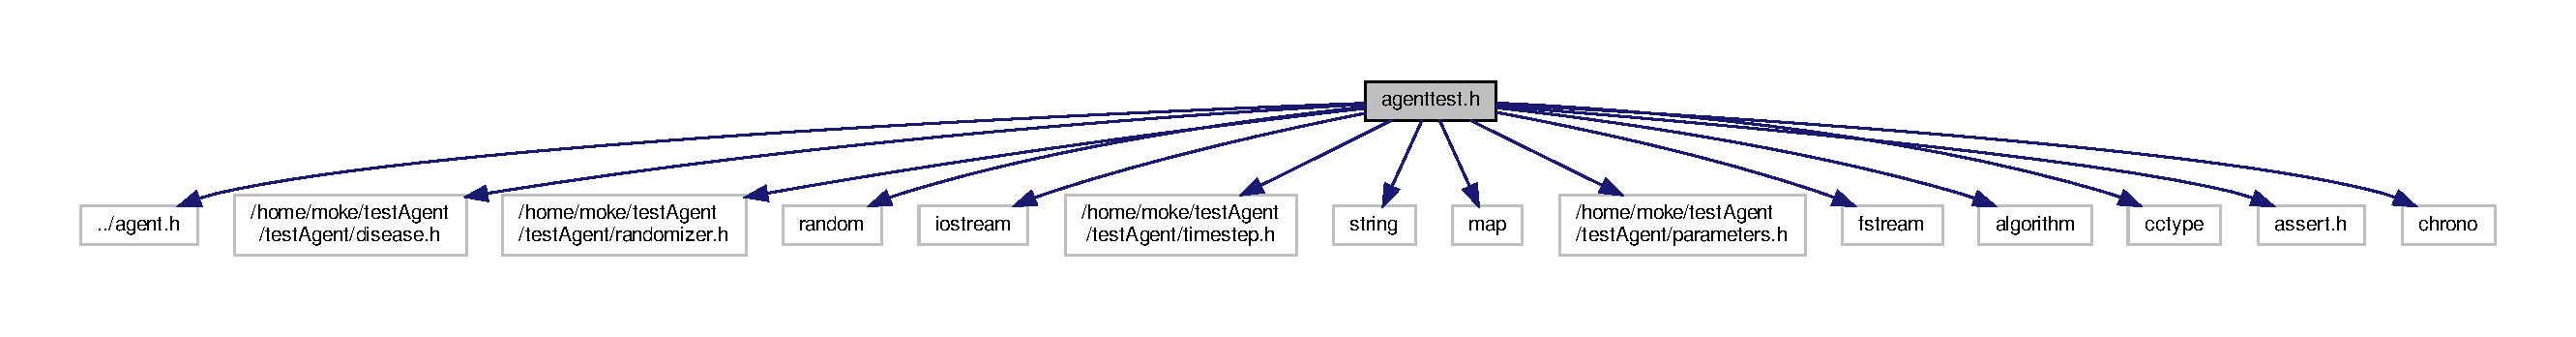
\includegraphics[width=350pt]{agenttest_8h__incl}
\end{center}
\end{figure}
This graph shows which files directly or indirectly include this file\+:\nopagebreak
\begin{figure}[H]
\begin{center}
\leavevmode
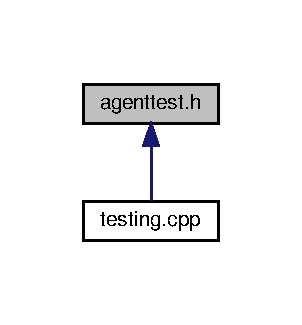
\includegraphics[width=145pt]{agenttest_8h__dep__incl}
\end{center}
\end{figure}
\subsection*{Classes}
\begin{DoxyCompactItemize}
\item 
class \mbox{\hyperlink{classagentTest}{agent\+Test}}
\begin{DoxyCompactList}\small\item\em test out the agent class \end{DoxyCompactList}\end{DoxyCompactItemize}


\subsection{Detailed Description}
File containing the definition of the \mbox{\hyperlink{classagentTest}{agent\+Test}} class. 

\begin{DoxyAuthor}{Author}
Mike Bithell 
\end{DoxyAuthor}
\begin{DoxyDate}{Date}
17/08/2021 
\end{DoxyDate}

\hypertarget{diseasetest_8h}{}\section{diseasetest.\+h File Reference}
\label{diseasetest_8h}\index{diseasetest.\+h@{diseasetest.\+h}}


File containing the definition of the \mbox{\hyperlink{classdiseaseTest}{disease\+Test}} class.  


{\ttfamily \#include \char`\"{}../disease.\+h\char`\"{}}\newline
Include dependency graph for diseasetest.\+h\+:\nopagebreak
\begin{figure}[H]
\begin{center}
\leavevmode
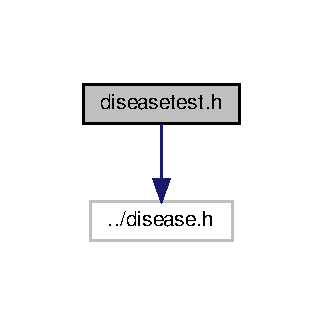
\includegraphics[width=155pt]{diseasetest_8h__incl}
\end{center}
\end{figure}
This graph shows which files directly or indirectly include this file\+:\nopagebreak
\begin{figure}[H]
\begin{center}
\leavevmode
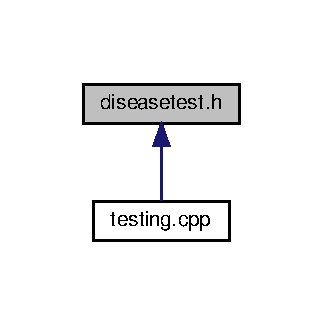
\includegraphics[width=155pt]{diseasetest_8h__dep__incl}
\end{center}
\end{figure}
\subsection*{Classes}
\begin{DoxyCompactItemize}
\item 
class \mbox{\hyperlink{classdiseaseTest}{disease\+Test}}
\begin{DoxyCompactList}\small\item\em test the disease static classs \end{DoxyCompactList}\end{DoxyCompactItemize}


\subsection{Detailed Description}
File containing the definition of the \mbox{\hyperlink{classdiseaseTest}{disease\+Test}} class. 

\begin{DoxyAuthor}{Author}
Mike Bithell 
\end{DoxyAuthor}
\begin{DoxyDate}{Date}
17/08/2021 
\end{DoxyDate}

\hypertarget{modelfactorytest_8h}{}\section{modelfactorytest.\+h File Reference}
\label{modelfactorytest_8h}\index{modelfactorytest.\+h@{modelfactorytest.\+h}}


File containing the definition of the \mbox{\hyperlink{classmodelFactoryTest}{model\+Factory\+Test}} class.  


{\ttfamily \#include \char`\"{}../model\+Factory.\+h\char`\"{}}\newline
Include dependency graph for modelfactorytest.\+h\+:
\nopagebreak
\begin{figure}[H]
\begin{center}
\leavevmode
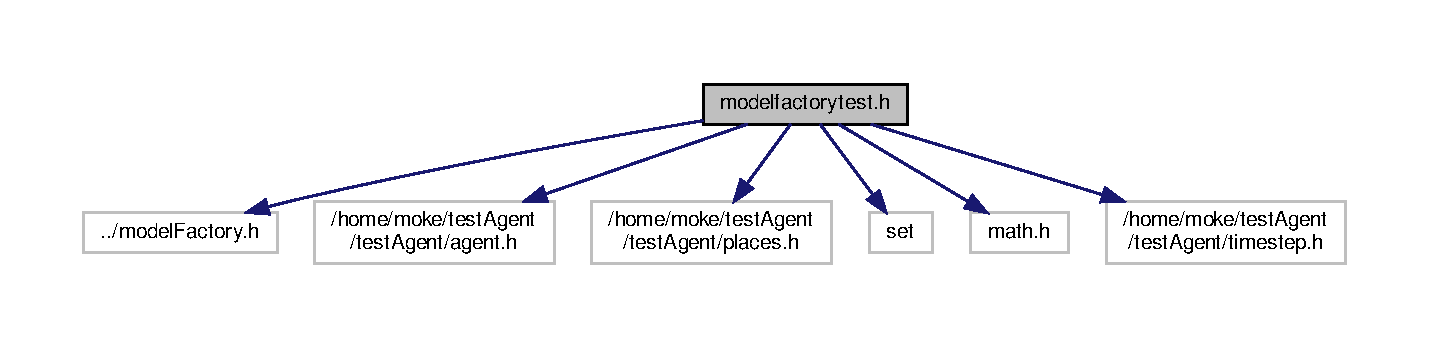
\includegraphics[width=350pt]{modelfactorytest_8h__incl}
\end{center}
\end{figure}
This graph shows which files directly or indirectly include this file\+:
\nopagebreak
\begin{figure}[H]
\begin{center}
\leavevmode
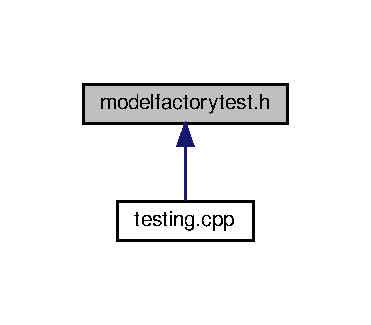
\includegraphics[width=178pt]{modelfactorytest_8h__dep__incl}
\end{center}
\end{figure}
\subsection*{Classes}
\begin{DoxyCompactItemize}
\item 
class \mbox{\hyperlink{classmodelFactoryTest}{model\+Factory\+Test}}
\begin{DoxyCompactList}\small\item\em test out the model\+Factory class \end{DoxyCompactList}\end{DoxyCompactItemize}


\subsection{Detailed Description}
File containing the definition of the \mbox{\hyperlink{classmodelFactoryTest}{model\+Factory\+Test}} class. 

\begin{DoxyAuthor}{Author}
Mike Bithell 
\end{DoxyAuthor}
\begin{DoxyDate}{Date}
17/08/2021 
\end{DoxyDate}

\hypertarget{modeltest_8h}{}\section{modeltest.\+h File Reference}
\label{modeltest_8h}\index{modeltest.\+h@{modeltest.\+h}}


File containing the definition of the \mbox{\hyperlink{classmodelTest}{model\+Test}} class.  


{\ttfamily \#include \char`\"{}../model.\+h\char`\"{}}\newline
{\ttfamily \#include $<$fstream$>$}\newline
Include dependency graph for modeltest.\+h\+:\nopagebreak
\begin{figure}[H]
\begin{center}
\leavevmode
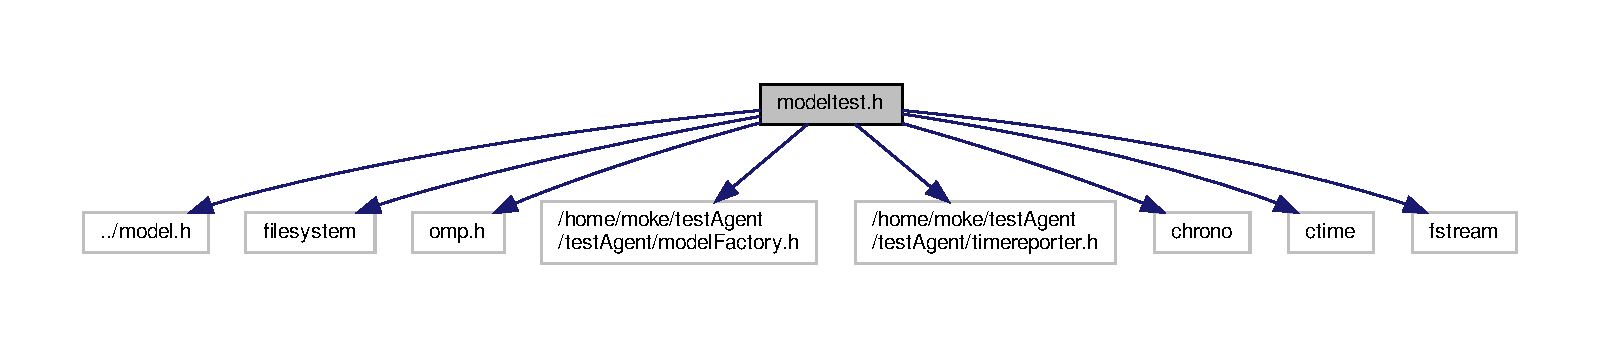
\includegraphics[width=350pt]{modeltest_8h__incl}
\end{center}
\end{figure}
This graph shows which files directly or indirectly include this file\+:\nopagebreak
\begin{figure}[H]
\begin{center}
\leavevmode
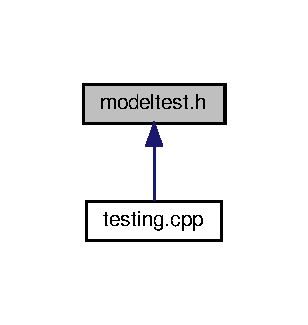
\includegraphics[width=148pt]{modeltest_8h__dep__incl}
\end{center}
\end{figure}
\subsection*{Classes}
\begin{DoxyCompactItemize}
\item 
class \mbox{\hyperlink{classmodelTest}{model\+Test}}
\begin{DoxyCompactList}\small\item\em test out the model class \end{DoxyCompactList}\end{DoxyCompactItemize}


\subsection{Detailed Description}
File containing the definition of the \mbox{\hyperlink{classmodelTest}{model\+Test}} class. 

\begin{DoxyAuthor}{Author}
Mike Bithell 
\end{DoxyAuthor}
\begin{DoxyDate}{Date}
17/08/2021 
\end{DoxyDate}

\hypertarget{parametertest_8h}{}\section{parametertest.\+h File Reference}
\label{parametertest_8h}\index{parametertest.\+h@{parametertest.\+h}}


File containing the definition of the \mbox{\hyperlink{classparameterTest}{parameter\+Test}} class for testing the parameter file.  


This graph shows which files directly or indirectly include this file\+:\nopagebreak
\begin{figure}[H]
\begin{center}
\leavevmode
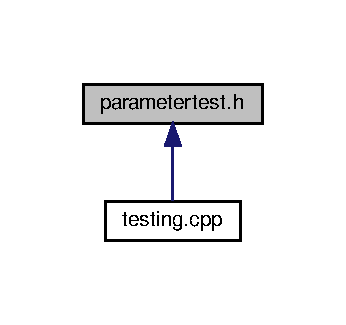
\includegraphics[width=166pt]{parametertest_8h__dep__incl}
\end{center}
\end{figure}
\subsection*{Classes}
\begin{DoxyCompactItemize}
\item 
class \mbox{\hyperlink{classparameterTest}{parameter\+Test}}
\begin{DoxyCompactList}\small\item\em Check parameter defaults are as expected. \end{DoxyCompactList}\end{DoxyCompactItemize}


\subsection{Detailed Description}
File containing the definition of the \mbox{\hyperlink{classparameterTest}{parameter\+Test}} class for testing the parameter file. 

\begin{DoxyAuthor}{Author}
Mike Bithell 
\end{DoxyAuthor}
\begin{DoxyDate}{Date}
17/08/2021 
\end{DoxyDate}

\hypertarget{placetest_8h}{}\section{placetest.\+h File Reference}
\label{placetest_8h}\index{placetest.\+h@{placetest.\+h}}


File containing the definition of the \mbox{\hyperlink{classplaceTest}{place\+Test}} class.  


{\ttfamily \#include \char`\"{}../places.\+h\char`\"{}}\newline
Include dependency graph for placetest.\+h\+:\nopagebreak
\begin{figure}[H]
\begin{center}
\leavevmode
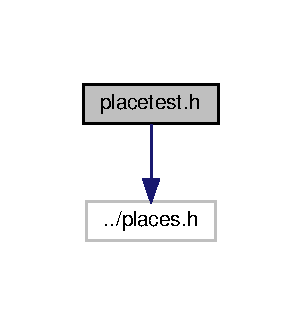
\includegraphics[width=145pt]{placetest_8h__incl}
\end{center}
\end{figure}
This graph shows which files directly or indirectly include this file\+:\nopagebreak
\begin{figure}[H]
\begin{center}
\leavevmode
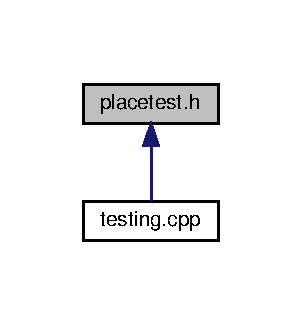
\includegraphics[width=145pt]{placetest_8h__dep__incl}
\end{center}
\end{figure}
\subsection*{Classes}
\begin{DoxyCompactItemize}
\item 
class \mbox{\hyperlink{classplaceTest}{place\+Test}}
\begin{DoxyCompactList}\small\item\em Check places for contamination levels and agent occupancy. \end{DoxyCompactList}\end{DoxyCompactItemize}


\subsection{Detailed Description}
File containing the definition of the \mbox{\hyperlink{classplaceTest}{place\+Test}} class. 

\begin{DoxyAuthor}{Author}
Mike Bithell 
\end{DoxyAuthor}
\begin{DoxyDate}{Date}
17/08/2021 
\end{DoxyDate}

\hypertarget{randomtest_8h}{}\section{randomtest.\+h File Reference}
\label{randomtest_8h}\index{randomtest.\+h@{randomtest.\+h}}


File containing the definition of the \mbox{\hyperlink{classrandomTest}{random\+Test}} class for the random number wrapper.  


{\ttfamily \#include \char`\"{}../randomizer.\+h\char`\"{}}\newline
Include dependency graph for randomtest.\+h\+:\nopagebreak
\begin{figure}[H]
\begin{center}
\leavevmode
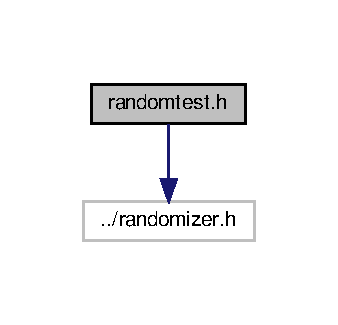
\includegraphics[width=162pt]{randomtest_8h__incl}
\end{center}
\end{figure}
This graph shows which files directly or indirectly include this file\+:\nopagebreak
\begin{figure}[H]
\begin{center}
\leavevmode
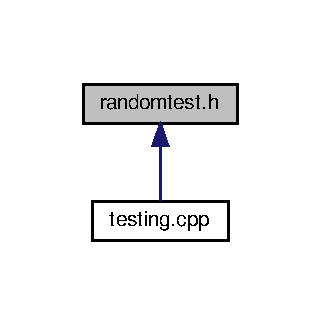
\includegraphics[width=154pt]{randomtest_8h__dep__incl}
\end{center}
\end{figure}
\subsection*{Classes}
\begin{DoxyCompactItemize}
\item 
class \mbox{\hyperlink{classrandomTest}{random\+Test}}
\begin{DoxyCompactList}\small\item\em Test some of the random number generator behaviour. \end{DoxyCompactList}\end{DoxyCompactItemize}


\subsection{Detailed Description}
File containing the definition of the \mbox{\hyperlink{classrandomTest}{random\+Test}} class for the random number wrapper. 

\begin{DoxyAuthor}{Author}
Mike Bithell 
\end{DoxyAuthor}
\begin{DoxyDate}{Date}
17/08/2021 
\end{DoxyDate}

\hypertarget{schedulelisttest_8h}{}\section{schedulelisttest.\+h File Reference}
\label{schedulelisttest_8h}\index{schedulelisttest.\+h@{schedulelisttest.\+h}}


File containing the definition of the newclass\+Test class.  


{\ttfamily \#include \char`\"{}../schedulelist.\+h\char`\"{}}\newline
Include dependency graph for schedulelisttest.\+h\+:
\nopagebreak
\begin{figure}[H]
\begin{center}
\leavevmode
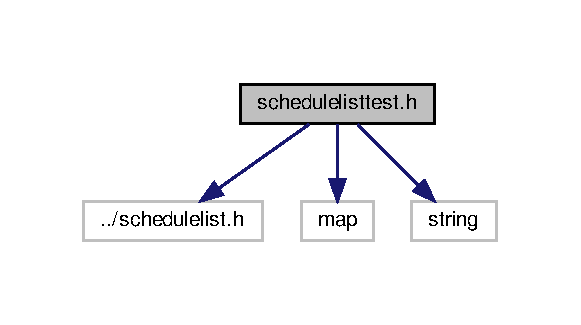
\includegraphics[width=279pt]{schedulelisttest_8h__incl}
\end{center}
\end{figure}
This graph shows which files directly or indirectly include this file\+:
\nopagebreak
\begin{figure}[H]
\begin{center}
\leavevmode
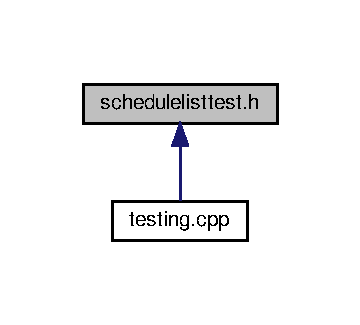
\includegraphics[width=173pt]{schedulelisttest_8h__dep__incl}
\end{center}
\end{figure}
\subsection*{Classes}
\begin{DoxyCompactItemize}
\item 
class \mbox{\hyperlink{classscheduleListTest}{schedule\+List\+Test}}
\begin{DoxyCompactList}\small\item\em test out the newclass class \end{DoxyCompactList}\end{DoxyCompactItemize}


\subsection{Detailed Description}
File containing the definition of the newclass\+Test class. 

\begin{DoxyAuthor}{Author}
Mike Bithell 
\end{DoxyAuthor}
\begin{DoxyDate}{Date}
27/10/2021 
\end{DoxyDate}

\hypertarget{testing_8cpp}{}\section{testing.\+cpp File Reference}
\label{testing_8cpp}\index{testing.\+cpp@{testing.\+cpp}}


Define the progress test listener, \mbox{\hyperlink{classMyCustomProgressTestListener}{My\+Custom\+Progress\+Test\+Listener}}, and the main function to run all the tests.  


{\ttfamily \#include $<$iostream$>$}\newline
{\ttfamily \#include $<$string$>$}\newline
{\ttfamily \#include $<$cppunit/\+Test\+Case.\+h$>$}\newline
{\ttfamily \#include $<$cppunit/\+Test\+Suite.\+h$>$}\newline
{\ttfamily \#include $<$cppunit/\+Test\+Caller.\+h$>$}\newline
{\ttfamily \#include $<$cppunit/ui/text/\+Test\+Runner.\+h$>$}\newline
{\ttfamily \#include $<$cppunit/\+Test\+Result.\+h$>$}\newline
{\ttfamily \#include $<$cppunit/extensions/\+Helper\+Macros.\+h$>$}\newline
{\ttfamily \#include $<$cppunit/\+Text\+Test\+Progress\+Listener.\+h$>$}\newline
{\ttfamily \#include \char`\"{}../agent.\+h\char`\"{}}\newline
{\ttfamily \#include $<$math.\+h$>$}\newline
{\ttfamily \#include \char`\"{}randomtest.\+h\char`\"{}}\newline
{\ttfamily \#include \char`\"{}timereportertest.\+h\char`\"{}}\newline
{\ttfamily \#include \char`\"{}timesteptest.\+h\char`\"{}}\newline
{\ttfamily \#include \char`\"{}travelscheduletest.\+h\char`\"{}}\newline
{\ttfamily \#include \char`\"{}schedulelisttest.\+h\char`\"{}}\newline
{\ttfamily \#include \char`\"{}diseasetest.\+h\char`\"{}}\newline
{\ttfamily \#include \char`\"{}placetest.\+h\char`\"{}}\newline
{\ttfamily \#include \char`\"{}parametertest.\+h\char`\"{}}\newline
{\ttfamily \#include \char`\"{}agenttest.\+h\char`\"{}}\newline
{\ttfamily \#include \char`\"{}modelfactorytest.\+h\char`\"{}}\newline
{\ttfamily \#include \char`\"{}modeltest.\+h\char`\"{}}\newline
Include dependency graph for testing.\+cpp\+:\nopagebreak
\begin{figure}[H]
\begin{center}
\leavevmode
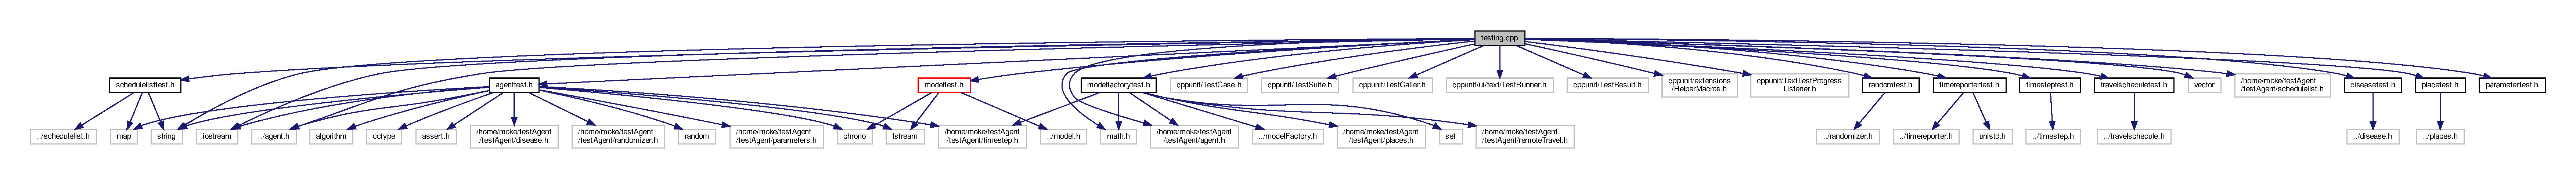
\includegraphics[width=350pt]{testing_8cpp__incl}
\end{center}
\end{figure}
\subsection*{Classes}
\begin{DoxyCompactItemize}
\item 
class \mbox{\hyperlink{classMyCustomProgressTestListener}{My\+Custom\+Progress\+Test\+Listener}}
\begin{DoxyCompactList}\small\item\em Report the start of each test. \end{DoxyCompactList}\end{DoxyCompactItemize}
\subsection*{Functions}
\begin{DoxyCompactItemize}
\item 
int \mbox{\hyperlink{testing_8cpp_ae66f6b31b5ad750f1fe042a706a4e3d4}{main}} ()
\begin{DoxyCompactList}\small\item\em Run the main set of test suites. \end{DoxyCompactList}\end{DoxyCompactItemize}


\subsection{Detailed Description}
Define the progress test listener, \mbox{\hyperlink{classMyCustomProgressTestListener}{My\+Custom\+Progress\+Test\+Listener}}, and the main function to run all the tests. 

\begin{DoxyAuthor}{Author}
Mike Bithell 
\end{DoxyAuthor}
\begin{DoxyDate}{Date}
17/08/2021 
\end{DoxyDate}


\subsection{Function Documentation}
\mbox{\Hypertarget{testing_8cpp_ae66f6b31b5ad750f1fe042a706a4e3d4}\label{testing_8cpp_ae66f6b31b5ad750f1fe042a706a4e3d4}} 
\index{testing.\+cpp@{testing.\+cpp}!main@{main}}
\index{main@{main}!testing.\+cpp@{testing.\+cpp}}
\subsubsection{\texorpdfstring{main()}{main()}}
{\footnotesize\ttfamily int main (\begin{DoxyParamCaption}{ }\end{DoxyParamCaption})}



Run the main set of test suites. 

First set up Test\+Runner then the Listener to report the start of each test. Then add the listener and each of the test suites to the Test\+Runner~\newline
Finally call the run method of Test\+Runner to execute all the test suites 
\hypertarget{timereportertest_8h}{}\section{timereportertest.\+h File Reference}
\label{timereportertest_8h}\index{timereportertest.\+h@{timereportertest.\+h}}


File containing the definition of the \mbox{\hyperlink{classtimeReporterTest}{time\+Reporter\+Test}} class for reporting run-\/time intervals.  


{\ttfamily \#include \char`\"{}../timereporter.\+h\char`\"{}}\newline
{\ttfamily \#include $<$unistd.\+h$>$}\newline
Include dependency graph for timereportertest.\+h\+:\nopagebreak
\begin{figure}[H]
\begin{center}
\leavevmode
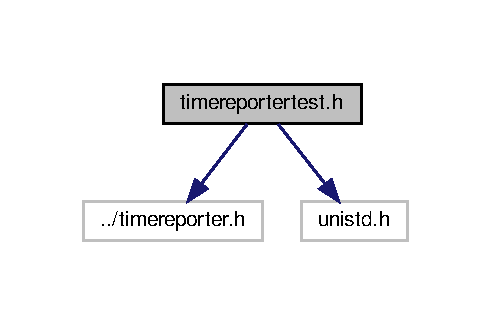
\includegraphics[width=236pt]{timereportertest_8h__incl}
\end{center}
\end{figure}
This graph shows which files directly or indirectly include this file\+:\nopagebreak
\begin{figure}[H]
\begin{center}
\leavevmode
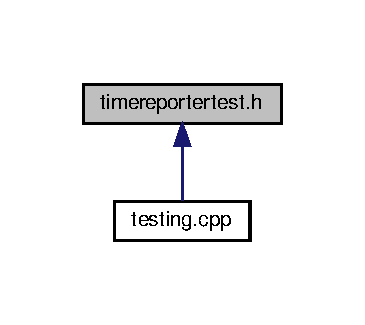
\includegraphics[width=175pt]{timereportertest_8h__dep__incl}
\end{center}
\end{figure}
\subsection*{Classes}
\begin{DoxyCompactItemize}
\item 
class \mbox{\hyperlink{classtimeReporterTest}{time\+Reporter\+Test}}
\begin{DoxyCompactList}\small\item\em Check intervals are computed and reported as expected. \end{DoxyCompactList}\end{DoxyCompactItemize}


\subsection{Detailed Description}
File containing the definition of the \mbox{\hyperlink{classtimeReporterTest}{time\+Reporter\+Test}} class for reporting run-\/time intervals. 

\begin{DoxyAuthor}{Author}
Mike Bithell 
\end{DoxyAuthor}
\begin{DoxyDate}{Date}
17/08/2021 
\end{DoxyDate}

\hypertarget{timesteptest_8h}{}\section{timesteptest.\+h File Reference}
\label{timesteptest_8h}\index{timesteptest.\+h@{timesteptest.\+h}}


File containing the definition of the \mbox{\hyperlink{classtimeStepTest}{time\+Step\+Test}} class for checking the time step to real world times class is working.  


{\ttfamily \#include \char`\"{}../timestep.\+h\char`\"{}}\newline
Include dependency graph for timesteptest.\+h\+:\nopagebreak
\begin{figure}[H]
\begin{center}
\leavevmode
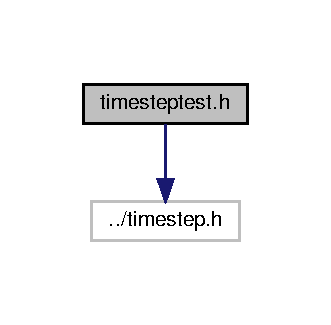
\includegraphics[width=159pt]{timesteptest_8h__incl}
\end{center}
\end{figure}
This graph shows which files directly or indirectly include this file\+:\nopagebreak
\begin{figure}[H]
\begin{center}
\leavevmode
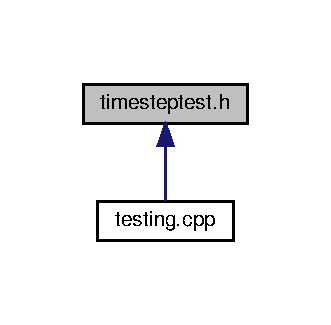
\includegraphics[width=159pt]{timesteptest_8h__dep__incl}
\end{center}
\end{figure}
\subsection*{Classes}
\begin{DoxyCompactItemize}
\item 
class \mbox{\hyperlink{classtimeStepTest}{time\+Step\+Test}}
\begin{DoxyCompactList}\small\item\em Check the class that maps the time step to a given set of real-\/world units (e.\+g. hours) \end{DoxyCompactList}\end{DoxyCompactItemize}


\subsection{Detailed Description}
File containing the definition of the \mbox{\hyperlink{classtimeStepTest}{time\+Step\+Test}} class for checking the time step to real world times class is working. 

\begin{DoxyAuthor}{Author}
Mike Bithell 
\end{DoxyAuthor}
\begin{DoxyDate}{Date}
17/08/2021 
\end{DoxyDate}

\hypertarget{travelscheduletest_8h}{}\section{travelscheduletest.\+h File Reference}
\label{travelscheduletest_8h}\index{travelscheduletest.\+h@{travelscheduletest.\+h}}


Test out the travel schedules using \mbox{\hyperlink{classtravelScheduleTest}{travel\+Schedule\+Test}} class.  


{\ttfamily \#include \char`\"{}../travelschedule.\+h\char`\"{}}\newline
Include dependency graph for travelscheduletest.\+h\+:\nopagebreak
\begin{figure}[H]
\begin{center}
\leavevmode
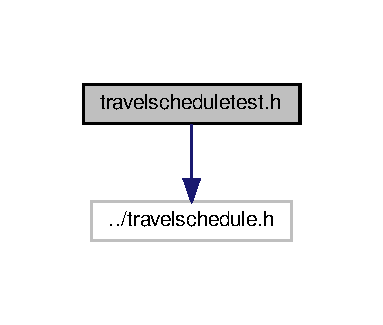
\includegraphics[width=184pt]{travelscheduletest_8h__incl}
\end{center}
\end{figure}
This graph shows which files directly or indirectly include this file\+:\nopagebreak
\begin{figure}[H]
\begin{center}
\leavevmode
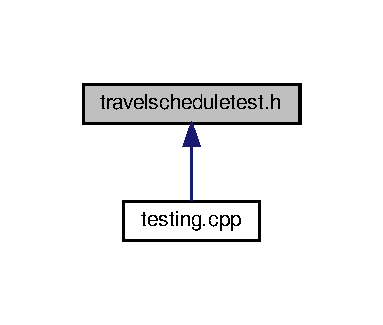
\includegraphics[width=184pt]{travelscheduletest_8h__dep__incl}
\end{center}
\end{figure}
\subsection*{Classes}
\begin{DoxyCompactItemize}
\item 
class \mbox{\hyperlink{classtravelScheduleTest}{travel\+Schedule\+Test}}
\begin{DoxyCompactList}\small\item\em Exercise the fixed travel schedules. \end{DoxyCompactList}\end{DoxyCompactItemize}


\subsection{Detailed Description}
Test out the travel schedules using \mbox{\hyperlink{classtravelScheduleTest}{travel\+Schedule\+Test}} class. 

\begin{DoxyAuthor}{Author}
Mike Bithell 
\end{DoxyAuthor}
\begin{DoxyDate}{Date}
17/08/2021 
\end{DoxyDate}

%--- End generated contents ---

% Index
\backmatter
\newpage
\phantomsection
\clearemptydoublepage
\addcontentsline{toc}{chapter}{Index}
\printindex

\end{document}
